\documentclass[a4paper,14pt]{report}

%%% Поля и разметка страницы %%%
\usepackage{lscape}		% Для включения альбомных страниц
\usepackage{geometry}	% Для последующего задания полей

%%% Кодировки и шрифты %%%
\usepackage{cmap}						% Улучшенный поиск русских слов в полученном pdf-файле
\usepackage[T2A]{fontenc}				% Поддержка русских букв
\usepackage[utf8]{inputenc}				% Кодировка utf8
\usepackage[english, russian]{babel}	% Языки: русский, английский
%\usepackage{pscyr}						% Красивые русские шрифты

\usepackage[fontsize=12]{scrextend}

%%% Математические пакеты %%%
\usepackage{amsthm,amsfonts,amsmath,amssymb,amscd} % Математические дополнения от AMS

%%% Оформление абзацев %%%
\usepackage{indentfirst} % Красная строка

%%%
\usepackage{misccorr}
\usepackage{setspace}

%%% Цвета %%%
\usepackage[usenames]{color}
\usepackage{color}
\usepackage{colortbl}

%%% Таблицы %%%
\usepackage{longtable}					% Длинные таблицы
\usepackage{multirow,makecell,array}	% Улучшенное форматирование таблиц

%%% Общее форматирование
%\usepackage[singlelinecheck=off,center]{caption}	% Многострочные подписи
\usepackage{soul}									% Поддержка переносоустойчивых подчёркиваний и зачёркиваний

%%% Библиография %%%
\usepackage{cite} % Красивые ссылки на литературу

%%% Гиперссылки %%%
\usepackage[unicode=true,linktocpage=true,plainpages=false,pdfpagelabels=false, pdftex]{hyperref}

%%% Изображения %%%
\usepackage{graphicx} % Подключаем пакет работы с графикой

%%% Оглавление %%%
\usepackage{tocloft}

% Подписи
%\usepackage{caption}
%\usepackage{subcaption}

% Верхняя подпись для таблицы
\usepackage{topcapt}

% Списки
\usepackage{enumitem}

\usepackage{afterpage}

\usepackage[russian]{nomencl}
%\usepackage{totcount}
%\usepackage{etoolbox}

\usepackage[nomargin,inline]{fixme}
%\usepackage{bibunits}

\usepackage{verbatim}

\usepackage{subfigure}
\usepackage{listingsutf8}

%\usepackage{slashbox}

\usepackage{fancyhdr}
                % Подключаемые пакеты
\hypersetup{
  pdftitle = {Mitel MX-ONE short manual},
  pdfauthor = {AM}
  }

%%% Макет страницы %%%
\geometry{a4paper,top=20mm,bottom=20mm,left=25mm,right=10mm}

%%% Кодировки и шрифты %%%
%\renewcommand{\rmdefault}{ftm} % Включаем Times New Roman

%%% Выравнивание и переносы %%%
\sloppy					% Избавляемся от переполнений
\clubpenalty=10000		% Запрещаем разрыв страницы после первой строки абзаца
\widowpenalty=10000		% Запрещаем разрыв страницы после последней строки абзаца

%%% Библиография %%%
%\bibliographystyle{ugost2008}
%\defaultbibliography{biblio}
%\makeatletter
%\bibliographystyle{utf8gost705u}	% Оформляем библиографию в
                                    % соответствии с ГОСТ 7.0.5
%\renewcommand{\@biblabel}[1]{\hfill#1.}	% Заменяем библиографию с
                                % квадратных скобок на точку: 
                                % без точки (АМ)
%\makeatother

% полуторный интервал (из пакета setspace)
\onehalfspacing

%%% Изображения %%%
\graphicspath{{images/}} % Пути к изображениям

% Подписи
%\DeclareCaptionLabelSeparator{tire}{~---~}
%\renewcommand{\thesubfigure}{\asbuk{subfigure}}  % рисунки а) б) в)
%\captionsetup{justification=centering,labelsep=tire}
%\captionsetup[table]{justification=left}

%%% Цвета гиперссылок %%%
\definecolor{linkcolor}{rgb}{0.1,0.1,0.6}
\definecolor{citecolor}{rgb}{0,0.6,0}
\definecolor{urlcolor}{rgb}{0,0,1}
\hypersetup{
    colorlinks, linkcolor={linkcolor},
    citecolor={citecolor}, urlcolor={urlcolor}
}

%%% Оглавление %%%
\renewcommand{\cftchapdotsep}{\cftdotsep}
 
% Списки
\makeatletter
    \AddEnumerateCounter{\asbuk}{\@asbuk}{м)}
\makeatother
\setlist{nolistsep}
\renewcommand{\labelitemi}{-}
\renewcommand{\labelenumi}{\asbuk{enumi})}
\renewcommand{\labelenumii}{\arabic{enumii})}

% Разделы c точкой на конце
%\renewcommand{\thechapter}{\arabic{chapter}}
%\renewcommand{\thesection}{\arabic{chapter}.\arabic{section}}
%\renewcommand{\thesubsection}{\arabic{chapter}.\arabic{section}.\arabic{subsection}}

\newcommand\Chapter[1]{
        \refstepcounter{chapter}
                \chapter*{
                \begin{huge}
                \textbf{\chaptername\ \arabic{chapter}\\}
                \end{huge}%
                \bigskip \bigskip
                \raggedright #1
        }
        \addcontentsline{toc}{chapter}{\arabic{chapter}. #1}
}

\newcommand\Section[1]{
        \refstepcounter{section}
        \section*{\raggedright
        \arabic{chapter}.\arabic{section} #1}
        \addcontentsline{toc}{section}{%
        \arabic{chapter}.\arabic{section}. #1}
}


\newcommand\Subsection[1]{
        \refstepcounter{subsection}
        \subsection*{\raggedright
        \arabic{chapter}.\arabic{section}.\arabic{subsection} #1}
        \addcontentsline{toc}{subsection}{%
        \arabic{chapter}.\arabic{section}.\arabic{subsection}. #1
        }
}

%%% Счётчики рисунков, таблиц и источников
\newcounter{totfigures}
\newcounter{tottables}
%\newcounter{totreferences}
%\makeatletter
%    \AtEndDocument{%
%      \addtocounter{totfigures}{\value{figure}}%
%      \addtocounter{tottables}{\value{table}}%
%      \immediate\write\@mainaux{%
%        \string\gdef\string\totfig{\number\value{totfigures}}%
%        \string\gdef\string\tottab{\number\value{tottables}}%
%        \string\gdef\string\totref{\number\value{totreferences}}%
%      }%
%    }
%\makeatother

%\pretocmd{\chapter}{\addtocounter{totfigures}{\value{figure}}}{}{}
%\pretocmd{\chapter}{\addtocounter{tottables}{\value{table}}}{}{}
%\pretocmd{\bibitem}{\addtocounter{totreferences}{1}}{}{}

% номенклатура
\makenomenclature

\lstloadlanguages{C,[GNU]C++,bash,Python,Awk,Gnuplot,Perl,tcl}
\lstset{
  basicstyle=\scriptsize,
  frame=tb,
%  backgroundcolor=\color{light-gray},
  commentstyle=\itshape,
  stringstyle=\bfseries,
  linewidth=\linewidth,
  breaklines=true,
  breakatwhitespace=true
}

%\captionsetup[lstlisting]{justification=left}
                  % Пользовательские стили

\begin{document}

%%% Переопределение именований %%%
\renewcommand{\abstractname}{Аннотация}
\renewcommand{\alsoname}{см. также}
\renewcommand{\appendixname}{Приложение}
\renewcommand{\bibname}{Ссылки}
\renewcommand{\ccname}{исх.}
\renewcommand{\chaptername}{Глава}
\renewcommand{\contentsname}{Содержание}
\renewcommand{\enclname}{вкл.}
\renewcommand{\figurename}{Рисунок}
\renewcommand{\headtoname}{вх.}
\renewcommand{\indexname}{Предметный указатель}
\renewcommand{\listfigurename}{Список рисунков}
\renewcommand{\listtablename}{Список таблиц}
\renewcommand{\pagename}{Стр.}
\renewcommand{\partname}{Часть}
\renewcommand{\refname}{Список литературы}
\renewcommand{\seename}{см.}
\renewcommand{\tablename}{Таблица}
\renewcommand{\nomname}{Обозначения и сокращения}
\renewcommand{\lstlistingname}{Листинг}
\renewcommand{\lstlistlistingname}{Список листингов}

\renewcommand{\le}{\leqslant}
\renewcommand{\ge}{\geqslant}
                   % Переопределение именований

\graphicspath{{img/}}
\thispagestyle{empty}

\begin{center}
МАЙТЕЛ
\end{center}

\vspace{30mm}

\vspace{30mm}
\begin{center}
{\bf Краткая инструкция по установке и настройке УПАТС MX--ONE\par}
\vspace{10mm}
{%\small
Версия 5.0 / 6.x
}
\end{center}

\vspace{20mm}
\begin{figure}[h]
  \center
    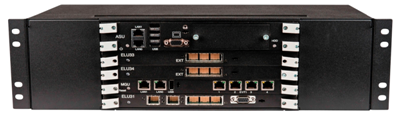
\includegraphics[width=0.5\linewidth]{mxone_lite}
    %\caption{}
    \label{img:mxone_lite}
\end{figure}

\vspace{50mm} \begin{center}
{Москва -- 2019}
\end{center}

%{\centering \em draft: \today}

\newpage
                   % Титульный лист

\tableofcontents
\clearpage
                % Оглавление

%\chapter*{Обозначения и сокращения}						% Заголовок
%\addcontentsline{toc}{chapter}{Обозначения и сокращения}	% Добавляем его в оглавление

\printnomenclature



\clearpage
               % Сокращения
%\printnomenclature
%\newpage

\pagestyle{fancy}
\fancyhead[CO,CE]{}
\fancyfoot[C]{\thepage}
\fancyfoot[L] {\tiny draft v1.3.4, Sep. 3, 2019} %\today}

%\input{introduction}            % Введение
\Chapter{Вводная часть} \label{chapter1}

Настоящая инструкция является кратким руководством по MX-ONE, за полным руководством следует обращаться к комплекту документации CPI. 
Описание компонентов системы и последние версии прошивок (firmware) для терминалов можно скачать с сайта Mitel \cite{miteldocs}. Для установки и настройки MX-ONE требуются базовые знания администрирования Linux, принципов IP--телефонии и прохождение учебных курсов Mitel MX--ONE. Дистрибутивы ПО MX--ONE доступны для скачивания прямым партнерам Mitel прошедшим соответствующую аттестацию.


\Section{Новые названия при переходе с версии 5.0 на версию 6.0} \label{sec:new_names}

\begin{table}[ht]
  \centering
  \topcaption{Старые и новые названия} \label{table:new_names}
  \begin{tabular}{ |*{2}{ p{8cm}| } }
    \hline
    Старое название в версии 5.0 & Новое название в версии 6.0 \\ \hline
    MX--ONE Telephony System (TS) & MiVoice MX--ONE Communication System (CS) \\ \hline
    MX--ONE Telephony Server (TSE) & MX--ONE Service Node (SN) \\ \hline
    MX--ONE Manager Provisioning (MP) & MX--ONE Provisioning Manager (PM) \\ \hline
    MX--ONE Manager Telephony System (MTS) & MX--ONE Service Node Manager (SNM) \\ \hline  
    MX--ONE Manager System Performance (MSP) & MX--ONE Traffic Manager (TM) \\ \hline
  \end{tabular}
\end{table}

\nomenclature{\ TS}{--- Telephony System (Телефонная система)}
\nomenclature{\ TSE}{--- Telephony Server (Телефонный сервер)}
\nomenclature{\ MTS}{--- Manager Telephony System (Управление телефонной системой)}
\nomenclature{\ MP}{--- Manager Provisioning (Управление пользователями)}

\nomenclature{\ CS}{--- Communication System (Коммуникационная система)}
\nomenclature{\ SN}{--- Service Node (Сервисный узел)}
\nomenclature{\ SNM}{--- Service Node Manager (Управление сервисным узлом)}
\nomenclature{\ PM}{--- Provisioning Manager (Управление пользователями)}

\nomenclature{\ ASU}{--- Advanced Server Unit (Улучшенный серверный модуль)}
\nomenclature{\ MGU}{--- Media Gateway Unit (Модуль медиа--шлюза)}
\nomenclature{\ MGW}{--- Media Gateway (Медиа--шлюз)}

\nomenclature{\ CPI}{--- Customer Product Information (Пользовательская документация о продукте)}

\section{Инсталляция MX--ONE}

Возможны несколько вариантов поставки MX--ONE:
\begin{itemize}
  \item MX-ONE может быть уже предустановлен на сервер ASU или Dell--сервер;
  \item в виде ISO--образа для установки, включающего в себя ПО MX--ONE и ОС SLES 10 \cite{sles};
  \item в виде готовой виртуальной машины (в виде OVA--файла) для VMWare ESXi 5.5 \cite{vmware};
  \item также ПО MX--ONE может устанавливаться на x86--сервер с предустановленной ОС SLES 10.
\end{itemize}
\nomenclature{\ SLES}{--- SUSE Linux Enterprise Server}
Требования к аппаратному обеспечению, в зависимости от планируемой нагрузки и кол-ва абонентов, приведены в документации CPI. 

\subsection{Установка на виртуальную машину из образа ISO}

Установка MX-ONE 5.0 из образа .iso на виртуальную машину VMWare:
\begin{enumerate}
\item Создать виртуальную машину (VM) SUSE Linux Enterprise 10 без установки ОС. 
\item Подключить .iso образ DVD к VM и запустить систему.
\nomenclature{\ VM}{--- Virtual Machine (Виртуальная машина)}
Если раздел на диске, куда будет устанавливаться система, занят другими данными, то его необходимо предварительно подготовить с помощь утилиты {\em fdisk}.

$\blacktriangleright$ {\em Пользоваться командой fdisk следует очень аккуратно, т.к. все данные на диске могут быть безвозвратно потеряны}.

В графическом меню загрузки с DVD выбрать пункт <<Rescue>> и загрузиться. Войти в Linux с именем {\em root}. Пароль на данном этапе не требуется.
Создать раздел на диске:
  \begin{lstlisting}
   #fdisk /dev/sda
  \end{lstlisting}
\par n - создать новый раздел
\par p - primary
\par 1 - первый раздел
\par по умолчанию выбрать цилиндры от первого до последнего
\par t - изменить тип раздела
\par b - тип FAT32
\par w - записать изменения и выйти
  \begin{lstlisting}
   #reboot 
  \end{lstlisting}
    
\item  В графическом меню загрузки с DVD выбрать пункт <<Installation>> и отредактировать Boot options:
\begin{lstlisting}
autoyast=file:///autoinst.xml
\end{lstlisting}

\end{enumerate}

Далее система установится автоматически.

В итоге при установке будут автоматически созданы и смонтированы новые разделы:

\begin{lstlisting}
# fdisk -l
Disk /dev/sda: 32.2 GB, 32212254720 bytes
255 heads, 63 sectors/track, 3916 cylinders
Units = cylinders of 16065 * 512 = 8225280 bytes

   Device Boot      Start         End      Blocks   Id  System
/dev/sda1   *           1          39      313236   83  Linux
/dev/sda2              40         301     2104515   82  Linux swap / Solaris
/dev/sda3             302        1868    12586927+  83  Linux
/dev/sda4            1869        3916    16450560    f  W95 Ext'd (LBA)
/dev/sda5            1869        2260     3148708+  83  Linux
/dev/sda6            2261        3916    13301788+  83  Linux

# df -h
Filesystem            Size  Used Avail Use% Mounted on
/dev/sda6              13G  7.1G  4.8G  60% /
udev                 1015M  128K 1014M   1% /dev
/dev/sda1             297M  9.9M  272M   4% /boot
/dev/sda5             3.0G  228M  2.6G   8% /eri_egx_root
/dev/sda3              12G  269M   11G   3% /var
\end{lstlisting}

\subsection{Файловая структура MX--ONE TSE}

$/opt/eri\_sn$ --- директория с поддиректориями с исполняемыми файлами приложений и шаблонами конфигурации (защищены от записи) \par
$/etc$ --- файлы для инсталляции и обновления конфигурации \par
$/etc/opt/eri\_sn$ --- активные конфигурационные файлы (доступны для записи) \par
$/var/opt/eri\_sn$ --- файлы с данными для перезагрузки и системный backup (доступны для записи) \par

\subsection{Инсталляция MX--ONE версии 5.0}

При первом запуске виртуальной машины необходимо настроить IP--адрес, имя хоста и доменное имя (рис. \ref{img:ip_config}).
\begin{figure}[ht]
  \center
  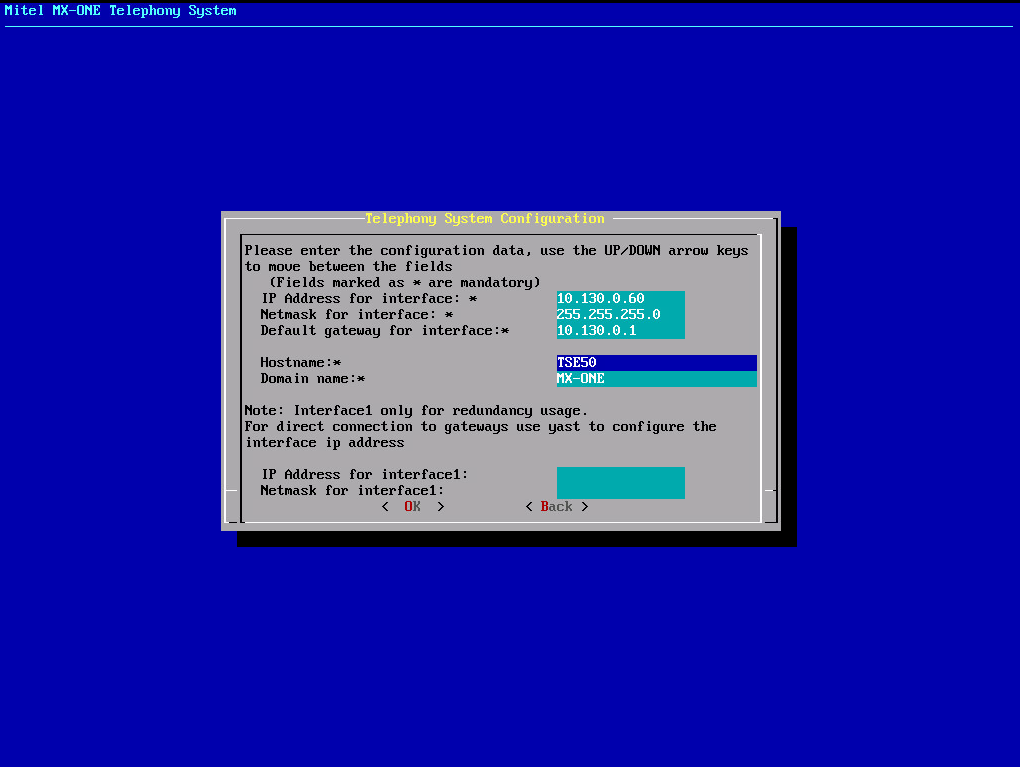
\includegraphics[width=\linewidth]{tse_ip_config}
  \caption{Настройка IP--адреса}
  \label{img:ip_config}
\end{figure}

$\blacktriangleright$ {\em Поменять IP--адрес после завершения процедуры инсталляции нельзя, для этого надо будет выполнить процедуру инсталляции заново}.

После загрузки системы к командной консоли CLI сервера MX--ONE можно подключиться через SSH--клиент. До момента окончания инсталляции системы к серверу можно подключиться с логином {\em root}. Логин и пароль по умолчанию для доступа через SSH:
\begin{lstlisting}
Login: eri_sn_admin
Password: Ericsson
\end{lstlisting}

$\blacktriangleright$ {\em Если в командной консоли перед командой стоит знак решетки <<\#>>, то команда выполняется от имени root, или знак << > >> в случае привилегированного пользователя}.

Если система устанавливается из образа ISO, то сначала устанавливается ОС Linux. После установки ОС необходимо запустить файл инсталляции MX--ONE от имени пользователя {\em root}:

\begin{lstlisting}
#sh /media/..../MX-ONE_install_verx.x.bin tk
\end{lstlisting}

Далее для настроек часового пояса (time zone) нужно запустить в командной консоли {\em yast} и выбрать в меню необходимую временную зону (\ref{img:yast_timezone}).
\begin{figure}[ht]
  \center
  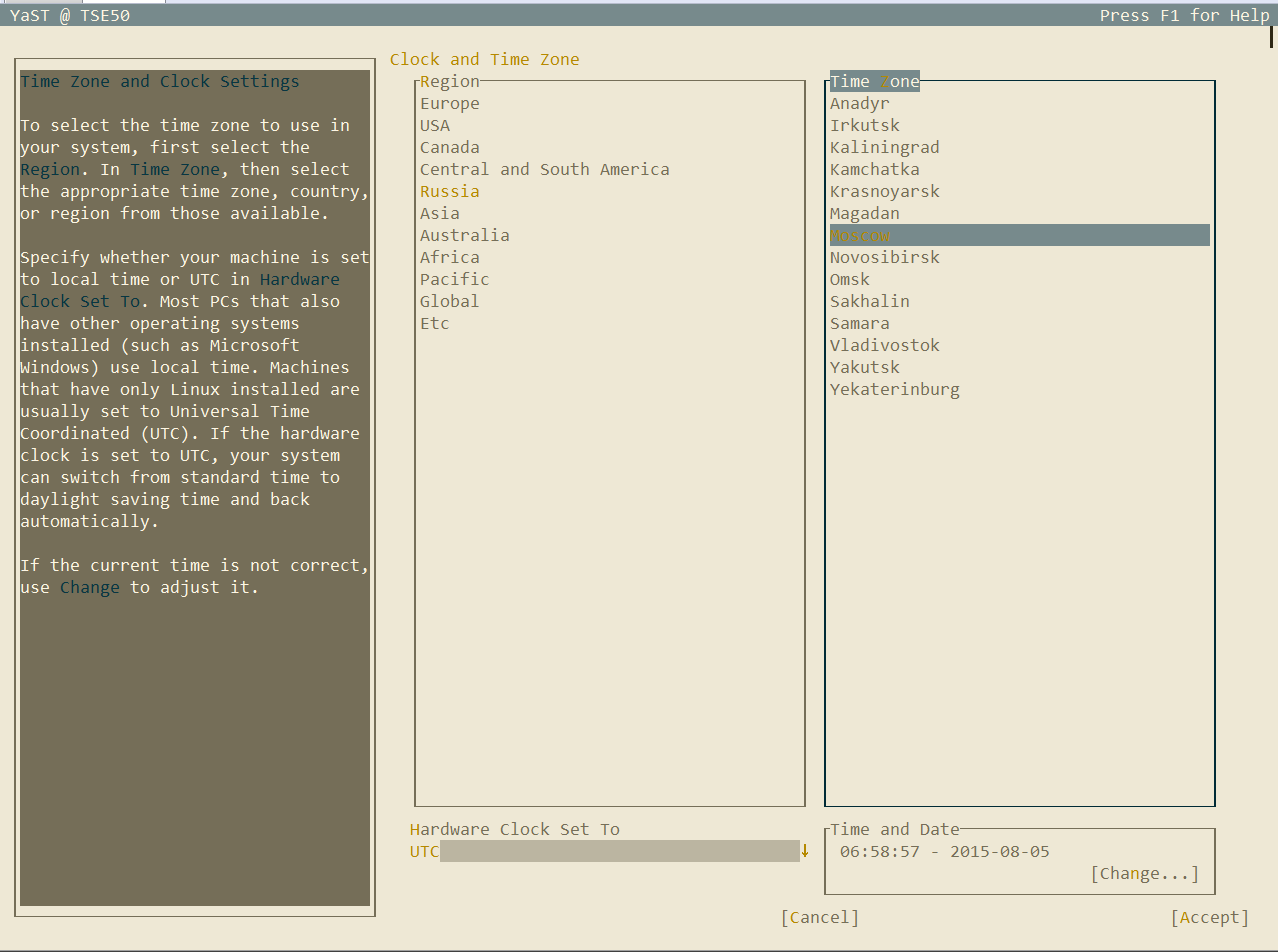
\includegraphics[width=\linewidth]{yast_timezone}
  \caption{YaST -- установка часового пояса}
  \label{img:yast_timezone}
\end{figure}

$\blacktriangleright$ {\em Язык системы должен быть по-умолчанию английский, менять его не нужно}.

После смены часового пояса необходимо перезагрузить систему:
\begin{lstlisting}
#reboot
\end{lstlisting}
\clearpage

Следующим шагом запускается настройка сервера MX-ONE TSE и веб--сервера MTS для настройки системы через графический интерфейс.
Команда в консоли {\em ts\_startup} от имени пользователя {\em root} запускает веб--сервер для конфигурации системы по IP--адресу \url{http://<ipaddress>/ICT/} (рис. \ref{img:ICT_general}).

\begin{figure}[ht]
  \center
  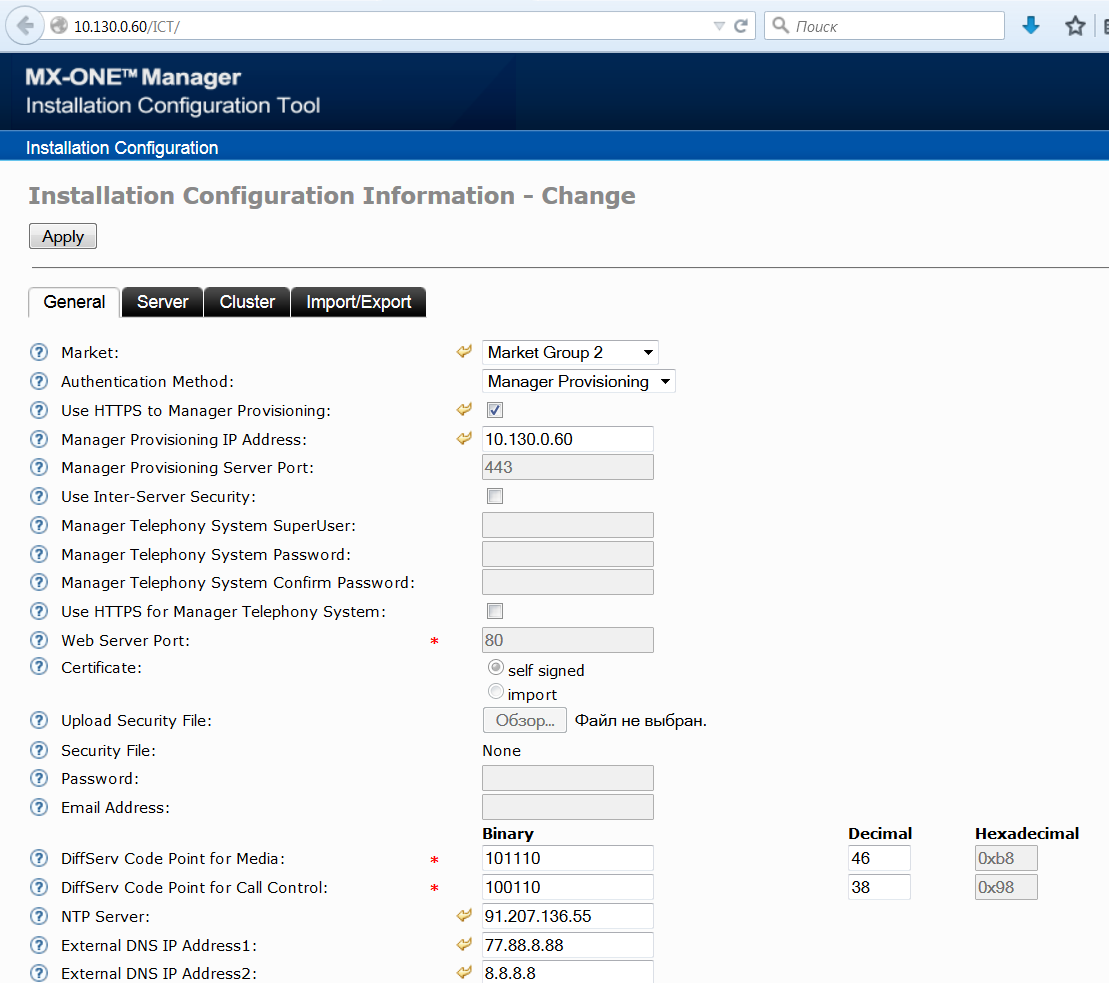
\includegraphics[width=\linewidth]{ICT_general}
  \caption{ICT -- настройка параметров системы}
  \label{img:ICT_general}
\end{figure}
\nomenclature{\ ICT}{--- Installation Configuration Tool (Инструмент для конфигурации инсталляции)}

На вкладке <<General>> для России и стран СНГ необходимо выбрать <<Market: Market Group 2>>. Метод аутентификации <<Linux account>> или <<Manager Provisioning>> если будет использоваться MP для входа в MTS. На этой же вкладке настраивается маркировка голосового и сигнального трафика DiffServ для обеспечения требуемого качества обслуживания (QoS). Подробнее об обеспечении качества передачи голоса в сетях IP можно прочитать в статьях \cite{yanovsky1, yanovsky2}.

Manager Provisioning по--умолчанию не входит в поставку, его нужно заказывать и устанавливать отдельно. Указываются адрес и порт сервера MP, если используется.

На вкладке <<Server>> нужно добавить настройки сервера TSE (рис. \ref{img:ICT_server}).
\begin{figure}[!ht]
  \center
  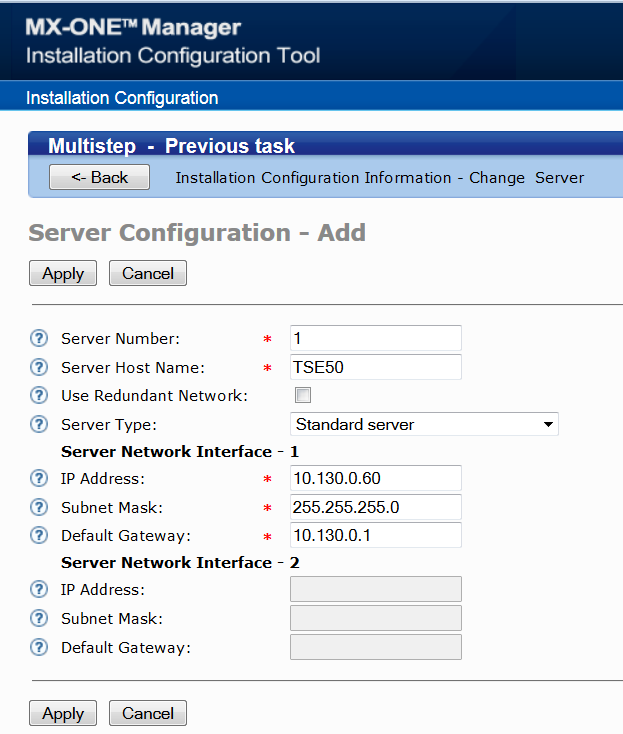
\includegraphics[width=0.6\linewidth]{ICT_server}
  \caption{ICT -- добавление сервера}
  \label{img:ICT_server}
\end{figure}
%\clearpage

На вкладке <<Cluster>> создаётся конфигурация кластера резервирования.
\par $\blacktriangleright$ {\em Кластер резервирования создаётся в момент инсталляции, изменить кластер потом без запуска инсталляции нельзя}.

На вкладке <<Import/Export>> можно загрузить или сохранить на диск конфигурацию системы (рис. \ref{img:ICT_export}).
\begin{figure}[!ht]
  \center
  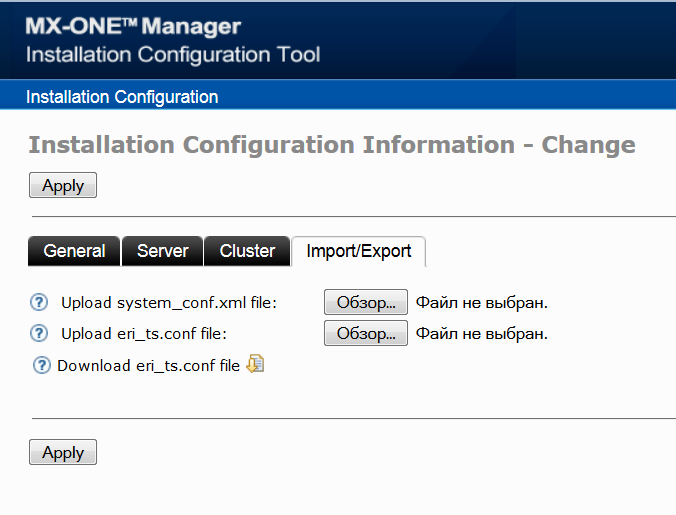
\includegraphics[width=0.6\linewidth]{ICT_export}
  \caption{ICT -- загрузка или сохраниение файлов конфигурации}
  \label{img:ICT_export}
\end{figure}

Конфигурация после настройки хранится в следующий файлах: 
\begin{lstlisting}
/etc/eri_ts.conf
/etc/system_conf.xml
\end{lstlisting}

После завершения настройки в веб--интерфейсе ICT, необходимо вернуться в консоль и нажать <<Enter>> для продолжения настройки и запуска TSE.

За процессом установки и сообщениями об возможных ошибках можно наблюдать открыв log--файл в другой консоли:
\begin{lstlisting}
eri_sn_admin@TSE50:~> tail -f /var/log/aastra/webserver/application_log.log
\end{lstlisting}

После окончания инсталляции должно быть выдано следующее сообщение об успешном завершении:
\begin{lstlisting}
The installation has finished successfully!
\end{lstlisting}

Версии установленного ПО MX--ONE доступны по команде {\em ts\_about}:
\begin{lstlisting}
eri_sn_admin@TSE50:~> ts_about
======  MX-ONE Telephony System  ======
Version: 5.0 SP6 build17

RPM Packages
============
Telephony Server 14.186 :
eri_sn-14.186-MR

Media Gateway File system 2.0 :
egx_rfs-2.0-1

Media Gateway 10.21 :
egx_sw-10.21-1

Media Gateway Classic 1.5.4 :
lsue_sw-1.5.4-1

Manager 9.316.18 :
   eri_om-9.316.18-201504201558
\end{lstlisting}

Базовые системные настройки теперь можно выполнить через графический интерфейс системы управления MTS, который доступен через веб--броузер по IP--адресу (или IP--адресу с добавлением имени {\em /mts}, если одновременно на той же машине установлен MP) \url{http://<ipaddress>/mts} (рис. \ref{img:mts_login}).
\begin{figure}[!ht]
  \center
  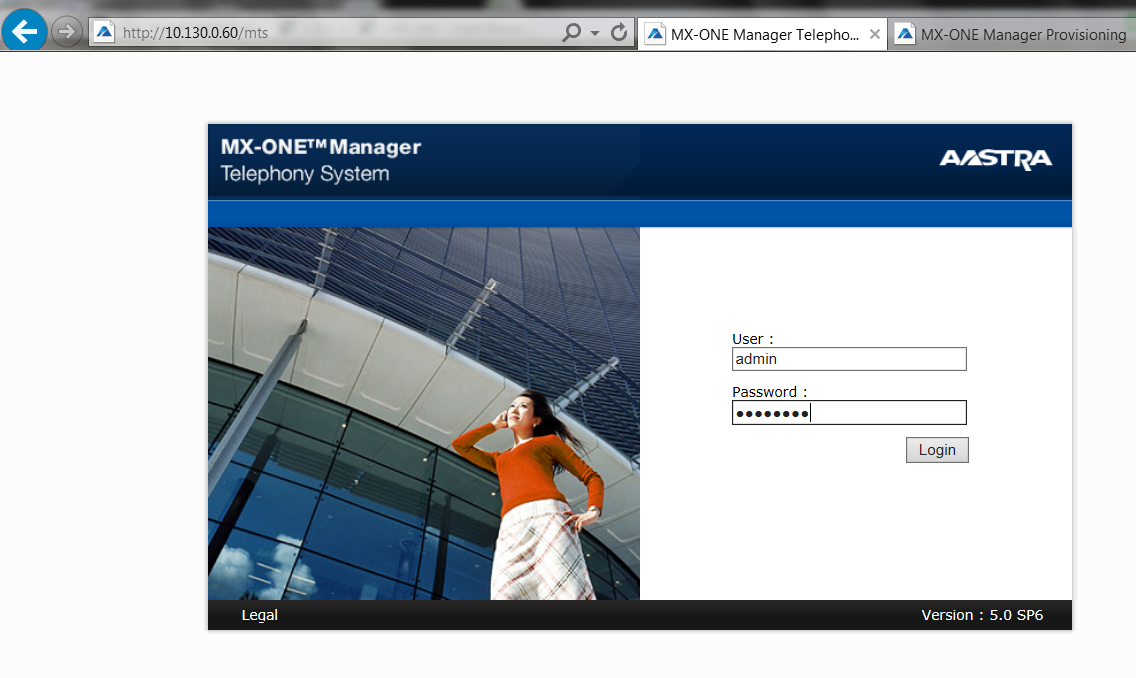
\includegraphics[width=\linewidth]{mts_login}
  \caption{Система управления Manager Telephony System}
  \label{img:mts_login}
\end{figure}
%\clearpage

Если для аутентификации в MTS используется учетная запись Linux, то этот пользователь должен быть включен в группу {\em snlev7} (рис. \ref{img:linux_user}).
\begin{figure}[!ht]
  \center
  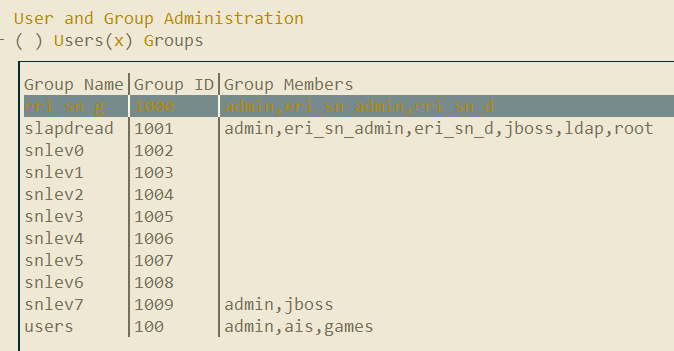
\includegraphics[width=0.7\linewidth]{linux_user}
  \caption{Настройка групп пользователей в YaST}
  \label{img:linux_user}
\end{figure}
%\clearpage

Дальше нужно создать в Manager Telephony System системные профайлы и номерной план (раздел \ref{sec:mts}).
Системные логи пишутся стандартно в файл {\em /var/log/messages}, а логи MX--ONE находятся в папке {\em /var/log/aastra/}.

После базовой настройки MX--ONE через CLI и web--интерфейс Manager Telephony System, рекомендуется установить также систему Manager Provisioning для настройки абонентов (раздел \ref{sec:mp}). 
\nomenclature{\ CLI}{--- Command Line Interface (Интерфейс командной строки)}

\clearpage

\subsection{Инсталляция MX--ONE версии 6.0}

MX--ONE 6.0 работает на базе операционной системы SLES 11 (64--bit) в отличие от SLES 10 (32--bit) для MX--ONE 5.0, и поэтому новую версию MX--ONE нельзя установить на ту же ОС. Процедура установки MX--ONE версии 6.0 также отличается от установки версии 5.0.

$\blacktriangleright$ {\em При каждой установке версии 6.0 создаётся новый уникальный {\em hardware id}, даже при повторной инсталляции на той же самой аппаратной платформе}.

В новой версии MX--ONE пароль по--умолчанию отсутствует, и теперь в процессе инсталляции необходимо задать пароли для 3--х пользователей (пароли должны быть одинаковыми для всех серверов в системе):
\begin{enumerate}
	\item root
	\item mxone\_admin
	\item mxone\_user
\end{enumerate}

$\blacktriangleright$ {\em Пароли не хранятся в системе в открытом виде и восстановить забытый пароль нельзя}.

Кластер резервирования теперь не обязательно создавать при инсталляции системы, в новой версии можно создать, изменить или удалить кластер в другое время при эксплуатации системы.

Дополнительно появился выбор модели лицензирования: произвольный выбор функций <<Traditional>> или выбор заранее определённых наборов <<Feature Based>>. Кроме того, можно сконфигурировать IPv6 адресацию.

$\blacktriangleright$ {\em Поменять параметры лицензирования и адресацию после завершения инсталляции нельзя}.

Вместо инструмента конфигурации {\em ICT} используется новый {\em network\_setup}. Для обслуживания системы также используется новый инструмент {\em mxone\_maintance}. 

\subsection{Установка Media Server}

MX-ONE поддерживает аудио--конференции до 8 участников, но для конференций используется ресурсы аппаратного модуля MGU или программный Media Server. Программный Media Server можно установить на тот же сервер MX-ONE или на отдельный, в зависимости от планируемой нагрузки.

Установка программного медиа--сервера выполняется от имени пользователя {\em root}:
\begin{lstlisting}
#rpm -ivh ./mgw-2.1.9-1.i386.rpm
\end{lstlisting}

Добавляем медиа--шлюз в систему c IP--адресом для управления:
\begin{lstlisting}
TSE50:# media_gateway_config -insert -mgw 1A -type MGU -ip 10.130.0.60 -gw 10.130.0.1

Setting media gateway control interface data:

Identity    Type  If no      Lim address      Ip address       Netmask      Default gateway  Name
1A       MGU      0      10.130.0.60      10.130.0.60        255.0.0.0       10.130.0.1


Are you sure? (Y/N): Y
END
\end{lstlisting}

Для RTP--трафика добавляем второй IP--адрес (alias) на тот же сетевой интерфейс с помощью {\em yast}: <<Network Devices>> $\rightarrow$ <<Network card>> $\rightarrow$ <<Edit>> $\rightarrow$ <<Advanced>> $\rightarrow$ <<Additional Address>> $\rightarrow$ <<Add>> (рис. \ref{img:ip_alias}). После этого настраиваем интерфейс медиа--шлюза на этот адрес:
\begin{figure}[!ht]
  \center
  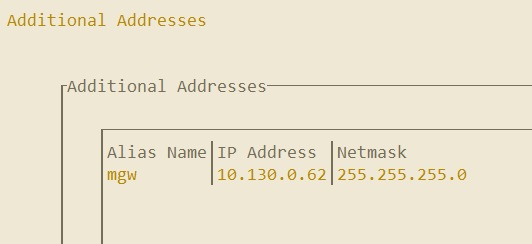
\includegraphics[width=0.7\linewidth]{ip_alias}
  \caption{YaST --- добавление второго IP--адреса}
  \label{img:ip_alias}
\end{figure}
%\clearpage


\begin{lstlisting}
  TSE50:# media_gateway_interface -mgw 1A -ip 10.130.0.62 -gw 10.130.0.1 -mask 255.255.255.0
  Setting data:
  Media interface   : number 0
  Interface address : 10.130.0.62
  Subnet Mask       : 255.255.255.0
  Network           : 10.130.0.0
  Broadcast         : 10.130.0.255
  Default gateway   : 10.130.0.1
  Link capability   : auto

  Are you sure? (Y/N): y

  1A: .   Media interface must be allocated on the same network as control interface
\end{lstlisting}

\subsection{Установка лицензии}

Сразу после установки системы, MX--ONE будет работать со временной лицензией. Для MX-ONE версии 5.0 --- 60 дней (1440 часов), для версии 6.0 --- 20 дней (480 часов). Лицензию и номер {\em hardware id} можно проверить с помощью команды {\em license\_status}: 
\begin{lstlisting}
eri_sn_admin@TSE50:~> license_status
Status on hardware id: 92816d-3e2832 (92816D-3E2832)
Licenced to hardware id 000000-000000
License file sequence number 0 with age 0 hours


Port licenses:
==============

                                          Tag     Trial time      Allowed         Used
=============================================   ============   ==========   ==========
                                    ACD-AGENT           1440            0         0

\end{lstlisting}

После истечения trial периода система заблокируется если не установить купленную лицензию.
Для установки лицензии необходимо скопировать полученный файл с лицензией:
\begin{lstlisting}
/etc/opt/eri_sn/lic.dat
\end{lstlisting}

и выполнить команду {\em license\_reread}. Лицензионный файл подходит только для системы с соответствующим {\em hardware id}.


\section{Настройка системных параметров в Manager Telephony System (MTS)} \label{sec:mts}


\subsection{Создание номерного плана} \label{subsec:numbers}

Создадим внутренние номера от 1000 до 2000 номера из главного меню MP:
{\em <<Number Analysis>> $\rightarrow$ <<Number Plan>> $\rightarrow$ <<Number Series>> $\rightarrow$ <<Add>> $\rightarrow$ <<Internal Numbers>>} (рис. \ref{img:number_series})
\begin{figure}[!ht]
  \center
  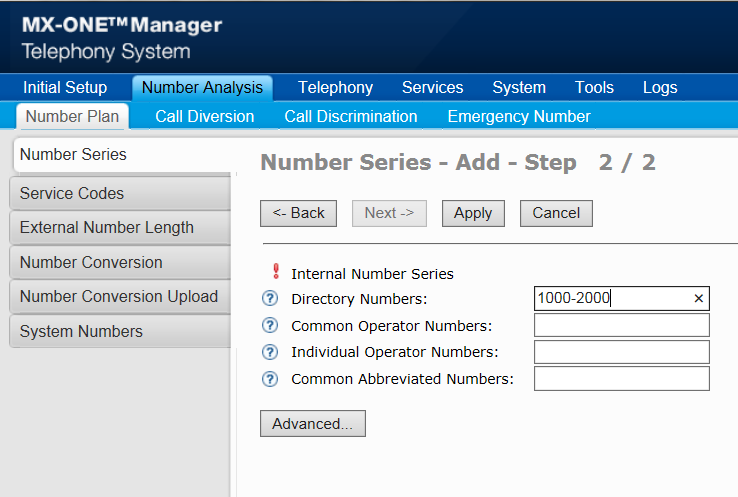
\includegraphics[width=0.7\linewidth]{number_series}
  \caption{Создание внутренних номеров в MTS}
  \label{img:number_series}
\end{figure}

\subsection{Создание группы одновременного вызова (Ring group)} \label{subsec:group}

Данная функция работает в MX--ONE только начиная с версии 6.0. В группу можно добавить до 16 номеров абонентов, которые будут звонить одновременно, и любой абонент из группы может ответить на вызов. Следующий вызов на ту же группу будет также распределен на свободных абонентов в группе. Если в группе все абоненты заняты, то новый вызов может ожидать в очереди, пока не появиться свободный абонент в группе или не истечет таймер ожидания.

Чтобы создать группу нужно войти в SNM (Service Node Manager) и перейти в меню: {\em <<Telephony>>  $\rightarrow$ <<Groups>> $\rightarrow$ <<Hunt Group>>} и создать новую группу, например со следующими параметрами (рис. \ref{img:hunt_group}):

\begin{lstlisting}
Directory Number:    110
Member Selection Order: Cascade
Maximum Number of Queuing Calls to the Group: 1
\end{lstlisting}

\begin{figure}[!ht]
  \center
  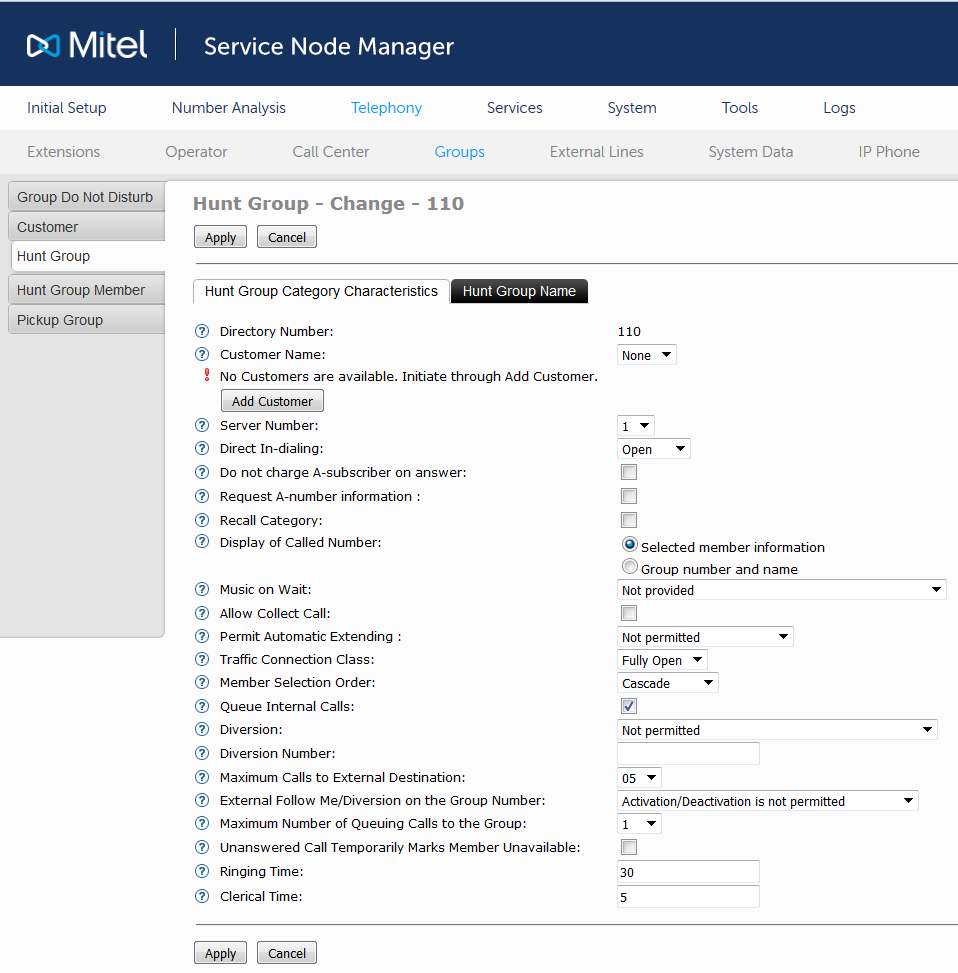
\includegraphics[width=0.9\linewidth]{hunt_group}
  \caption{Создание новый группы в SNM}
  \label{img:hunt_group}
\end{figure}

Далее в эту группу можно добавить номера абонентов через меню: {\em <<Telephony>>  $\rightarrow$ <<Groups>> $\rightarrow$ <<Hunt Group Member>>} рис. \ref{img:hunt_group_member}:

\begin{figure}[!ht]
  \center
  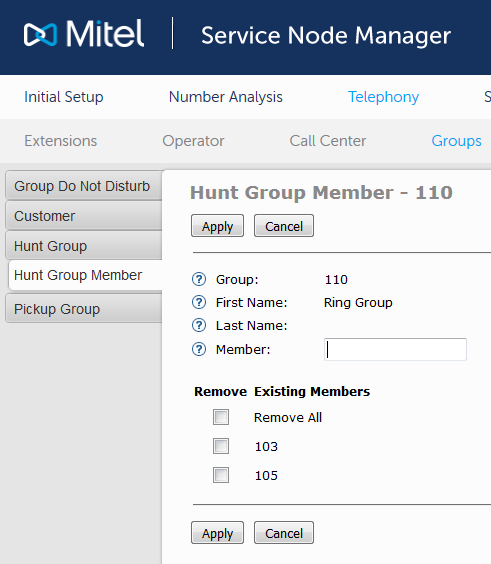
\includegraphics[width=0.6\linewidth]{hunt_group_member}
  \caption{Добавление абонентов в группу}
  \label{img:hunt_group_member}
\end{figure}
\clearpage

\subsection{Создание сервисного профайла} \label{subsec:csp}

Из главного меню добавляем новый профайл: {\em <<Telephony>> $\rightarrow$ <<Extensions>> $\rightarrow$ <<Common Service Profiles>> $\rightarrow$ <<Add>>} и вводим имя и номер профайла (рис. \ref{img:csp_identity}).
\begin{figure}[!ht]
  \center
  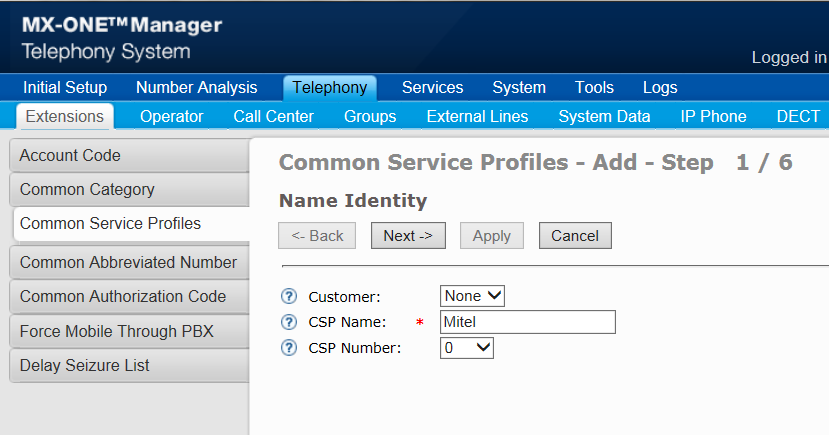
\includegraphics[width=0.8\linewidth]{csp_identity}
  \caption{Добавление нового сервисного профайла в MTS}
  \label{img:csp_identity}
\end{figure}

Далее проходим по настройкам и в конце подтверждаем создание профайла. В итоге должен появиться в списке новый профайл (\ref{img:csp_result}).
\begin{figure}[!ht]
  \center
  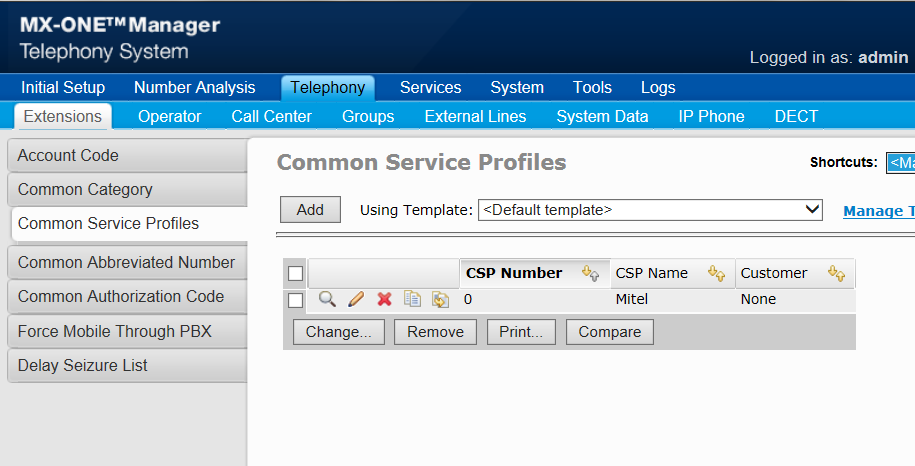
\includegraphics[width=0.8\linewidth]{csp_result}
  \caption{Новый сервисный профайл}
  \label{img:csp_result}
\end{figure}
\clearpage

\subsection{Создание маршрутов}

Для создания SIP--маршрута необходимо инициализировать категорию и данные маршрута. Нужно перейти в командную оболочку MD--shell с помощью команды $mdsh$ и выполнить команды $ROCAI$ c параметрами:
\begin{lstlisting}
MDSH> ROCAI:ROU=1,SEL=7110000000000010,SIG=0111110000A0,TRAF=03151515,\
  TRM=4,SERV=3100000001,BCAP=001100;
MDSH> RODAI:ROU=1,TYPE=TL66,VARC=00000000,VARI=00000000,VARO=00000000
\end{lstlisting}

В данном примере инициализируется SIP--маршрут (тип <<TL66>>) с номером 1. Для маршрута ISDN-E1 используется тип <<SL60>>. 

Далее можно описать SIP--маршрут командой {\em sip\_route -set} в Linux: 
\begin{lstlisting}
# sip_route -set -route 1 -uristring0 sip:?@192.168.222.197 -remoteport 5060 -fromuri0 sip:?@192.168.222.156 -protocol tcp
# sip_route -set -route 1 -accept REMOTE_IP -match 192.168.222.197
\end{lstlisting}
Указываются IP--адрес и порт удалённого SIP--сервера, исходящий адрес и используемый протокол. Второй командой разрешается приём соединений с указанного удалённого адреса.

Проверить данные маршрута можно командой {\em sip\_route -print -route 1}.

В завершении конфигурации необходимо инициализировать оборудование маршрута 1 в {\em mdsh}:
\begin{lstlisting}
MDSH> ROEQI:ROU=1,TRU=1-1;
\end{lstlisting}

Посмотреть информацию о маршрутах и категориях можно командами: 
\begin{lstlisting}
MDSH> rodap:rou=all;
MDSH> rocap:rou=all;
\end{lstlisting}

Добавление кода доступа 99 к маршруту 1 c передачей номера начиная с 3 цифры выполняется следующей командой:
\begin{lstlisting}
MDSH> RODDI:ROU=1,DEST=99,ADC=0005000000000250000001010000,SRT=3;
\end{lstlisting}

Просмотр информации о кодах доступа осуществляется командой:
\begin{lstlisting}
MDSH> roddp:dest=all;  
\end{lstlisting}

$\blacktriangleright$ {\em Назначение битов в параметрах команд описано в документации CPI. Необходимые для реального подключения значения параметров могут отличаться от приведённых в данном примере настройки маршрута}. 

Настройку внешних соединительных линий также можно выполнить в графическом интерфейсе MTS через меню: {\em <<Telephony>> $\rightarrow$ <<External Lines>> $\rightarrow$ <<Route>> $\rightarrow$ <<Add>>}. Пример настройки SIP--trunk приведён на рис. \ref{img:sip_trunk} и настройки ISDN-E1 на рис. \ref{img:isdn_trunk} соответственно.

\begin{figure}[!ht]
  \center
  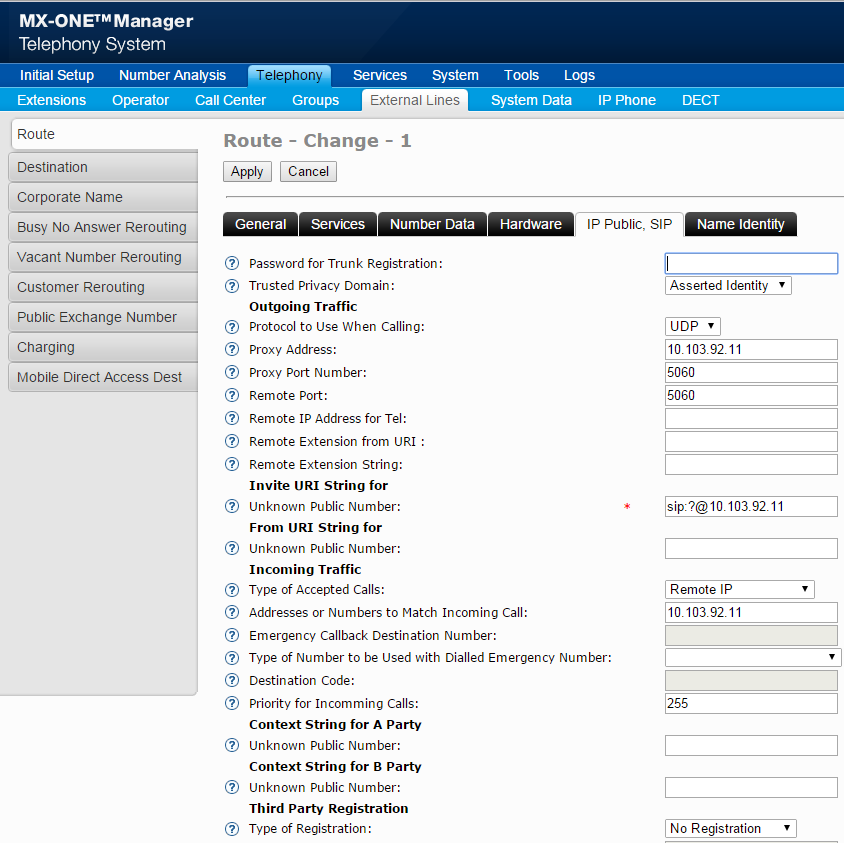
\includegraphics[width=\linewidth]{sip_trunk}
  \caption{Создание маршрута SIP в MTS}
  \label{img:sip_trunk}
\end{figure}

\begin{figure}[!ht]
  \center
  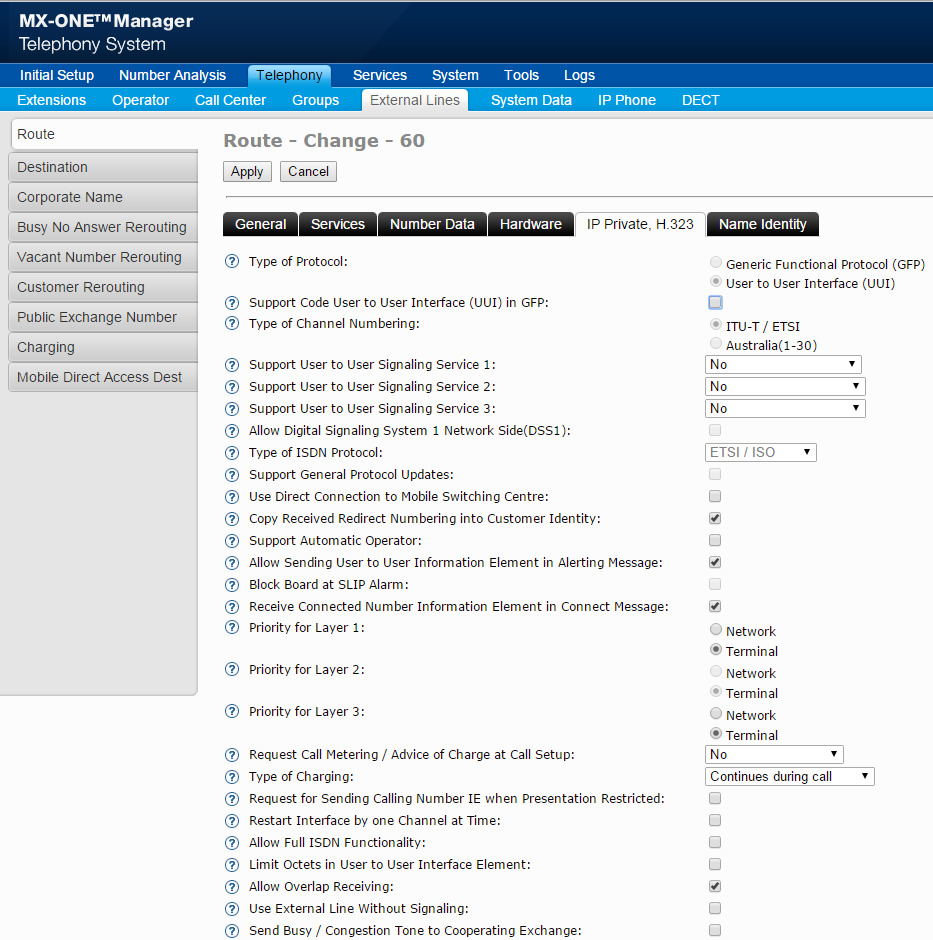
\includegraphics[width=\linewidth]{isdn_trunk}
  \caption{Создание маршрута ISDN-E1 в MTS}
  \label{img:isdn_trunk}
\end{figure}
\clearpage

\subsection{Создание резервных копий конфигурации}

Чтобы сделанные изменения сохранились после перезагрузки станции, необходимо сохранить конфигурации в файлах. Это можно сделать через графический интерфейс MTS в меню: {\em <<System>> $\rightarrow$ <<Backup \& Restore>>} (рис. \ref{img:backup})
\begin{figure}[!ht]
  \center
  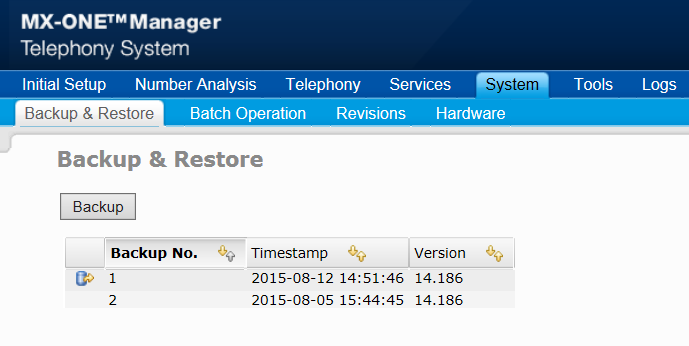
\includegraphics[width=0.7\linewidth]{backup}
  \caption{Создание и восстановление резервной копии конфигурации в MTS}
  \label{img:backup}
\end{figure}

В этом же меню можно восстановить предыдущую сохраненную конфигурацию нажав на изображение рядом с номером backup. 

Сохранить данные конфигурации можно также командой {\em data\_backup} в CLI:
\begin{lstlisting}
admin@TSE50:~> data_backup
Backup of exchange data

Backup of exchange data successful
\end{lstlisting}
Восстановить можно командой  {\em data\_restore}.

Последний backup используется для загрузки конфигурации при старте системы.

Сохраненные конфигурации хранятся в файлах на диске в директории {\em /var/opt/eri\_sn} в поддиректориях с именами {\em xdata\_y\_z}, где $y$ --- номер TSE, а $z$ --- дата создания резервной копии:

\begin{lstlisting}
TSE50:/ # ls -1 /var/opt/eri_sn/
.programpackageid.dat
call_logging
ldap
traffic_recording
usage_reports
xdata_1.conf
xdata_1_20150805154445
xdata_1_20150812145146
xdata_1_20150812145950
\end{lstlisting}

Если система состоит из нескольких серверов, то командой {\em config\_mirror} все конфигурации и резервные копии всех серверов копируются в директорию {\em /eri\_sn/mirror} на главный сервер TSE 1. Обратное действие производиться командой {\em config\_restore}.

Команда {\em eri\_sn\_safity\_backup} делает резервную копию конфигурационных файлов в один tar--файл в заданную директорию для хранения копии на отдельном носителе. Рекомендуется настроить через Linux--сервис {\em crontab} регулярное создание резервных конфигураций и копирование их на отдельный носитель в моменты времени с минимальной нагрузкой.

После восстановления конфигурации из резервной копии необходимо сделать координационный старт системы командой $start\ --system$ и потом выполнить рестарт $restart\ --system$ (раздел \ref{sec:restart}). 

Подробное описание процесса создания и восстановления резервных копий можно найти в CPI в Руководстве Администратора \cite{admin_guide} в разделе <<Backup \& Restore>>.
\clearpage 


\section{Администрирование системы}

\subsection{Преобразование номера}

Если при входящем звонке вызываемый номер совпадает с номером внутреннего абонента, то станция автоматически маршрутизирует вызов на внутреннего абонента. Если необходимо маршрутизировать вызов на определенного абонента с другим внутренним номером, то можно воспользоваться преобразованием номера. 

При входящем звонке для преобразования номера вызываемого абонента (B--номера) во внутренний номер используется команда {\em number\_conversion\_initiate} c опцией {\em -convertiontype 0}:
\begin{lstlisting}
> number_conversion_initiate  -entry XXXXXXX  -conversiontype 0  -route 1  -pre 1000  -numbertype 0  -truncate 7
\end{lstlisting}

В данном примере мы изменяем B--номер ХХХХХХХ удаляя 7 цифр (опция truncate) и добавляем внутренний номер 1000 для маршрута 1 (опция route).

При исходящем звонке для преобразования номера звонящего абонента (А--номера) во внешний номер, используется команда {\em number\_conversion\_initiate} c опцией {\em -convertiontype 1}:
\begin{lstlisting}
> number_conversion_initiate  -entry 1000  -conversiontype 1  -route 1  -pre XXXXXXX  -numbertype 10  -truncate 4
\end{lstlisting}

В этом примере мы удаляем 4 цифры A--номера 1000 и добавляем номер XXXXXXX.

\subsection{Настройка диапазона RTP--портов на MGU}

Настроить диапазон RTP/UDP--портов можно через MTS в меню {\em <<System>> $\rightarrow$ <<Hardware>> $\rightarrow$ <<Media Gateway>>} (рис. \ref{img:rtp_ports})
\begin{figure}[!ht]
  \center
  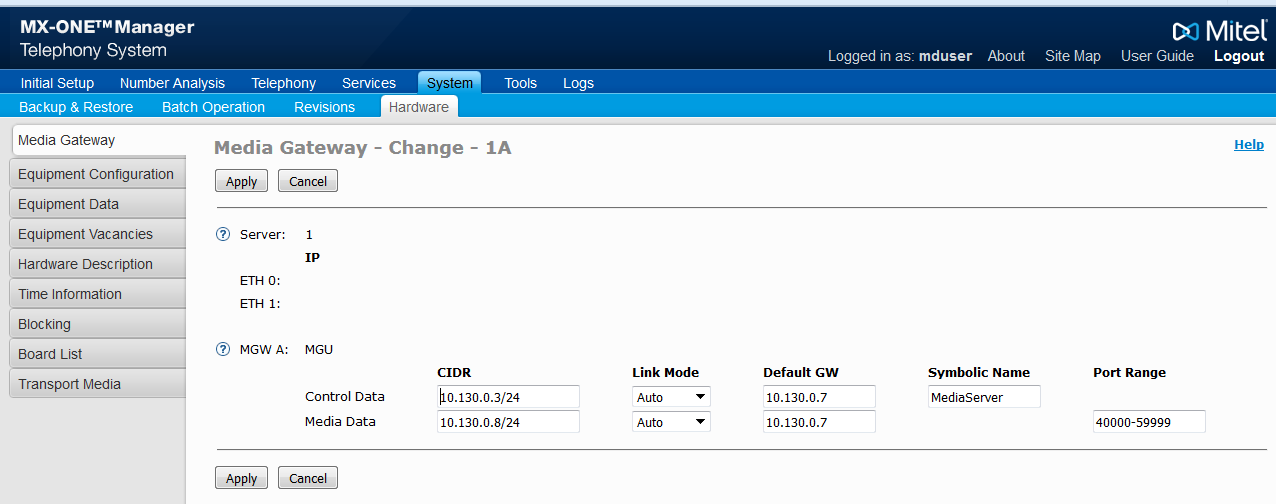
\includegraphics[width=\linewidth]{rtp_ports}
  \caption{Настройка RTP--портов на MGU}
  \label{img:rtp_ports}
\end{figure}

Посмотреть доступные RTP--ресурсы можно также с помощью команды через СLI {\em rtp\_resource}: 
\begin{lstlisting}
mxone_admin@MX-One6:~> rtp_resource
Identity  Local ip address  Port number range    Blocked  Busy  Max
MGW 1A    10.130.0.8           40000 - 59999     0        0     2000
Total:                                           0        0     2000
\end{lstlisting}
В данном примере показаны ресурсы программного медиа--сервера.

\subsection{Перенаправление голосового трафика через MGU} \label{subsec:forced}

Для некоторых приложений пассивной записи разговоров требуется, чтобы все звонки (RTP--потоки) проходили через MGU. В этом случае на каждый звонок между внутренними абонентами на MGU будут заниматься 2 RTP--ресурса.

$\blacktriangleright$ {\em Кол-во RTP--ресурсов в одном MGU ограничено: для MGU --- 256 RTP, для MGU2 --- 128 RTP, для программного Media Server до 2000}. 

Чтобы не занимать ресурсы MGU возможно использовать активный режим записи разговоров с интеграцией сервера записи по протоколу CSTA, при котором копии RTP--потоков записываются непосредственно с SIP--аппаратов по соответствующей команде с сервера. SIP--телефоны Mitel серии 6700/6800 могут по запросу отправлять копии RTP--потоков на сервер записи напрямую.

Для включения перенаправления трафика необходимо задать параметр «forced gateway» на MX--ONE. Это выполняется командой {\em extension\_profile} с параметром $--ext-serv$ и установкой бита 17 в значение <<1>>:
\begin{lstlisting}
D17 Unconditional forced Gateway: 
0 - no (default)
1 - yes
States whether all the calls to/from IP extensions will be unconditionally forced gateway
\end{lstlisting}

Данную опцию также можно включить через web--интерфейс MTS (SNM) в меню: {\em <<Telephony>> $\rightarrow$ <<Extensions>> $\rightarrow$ <<Common System Profiles>> $\rightarrow$ <<Service Category>>} отметить опцию <<Forced Calls from or to IP terminals to be Gateway Calls>> (рис. \ref{img:force_calls}):
\begin{figure}[!ht]
  \center
  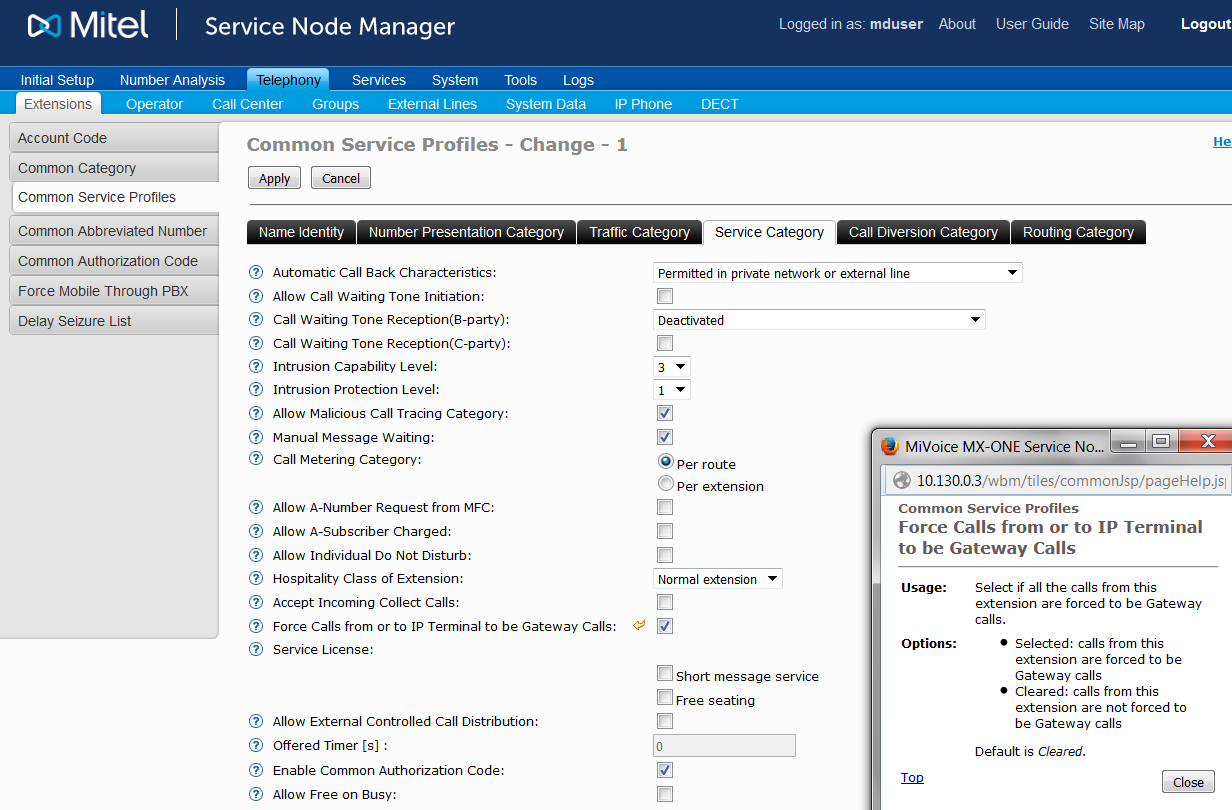
\includegraphics[width=\linewidth]{force_calls}
  \caption{Перенаправление RTP--потоков через медиа--шлюз}
  \label{img:force_calls}
\end{figure}

Проверить прохождение голосового трафика через шлюз можно с помощью трассировки вызова \ref{subsec:trace}.

\subsection{Резервирование сервера}

В MX-ONE 5.0 для резервирования серверов (TS) используется технология \href{http://www.linux-ha.org/doc/users-guide/users-guide.html}{Linux--HA}.

$\blacktriangleright$ {\em В MX-ONE 6.0 вместо Linux--HA используется технология резервирования собственной разработки}.

Для изменения значения таймеров Linux--HA по умолчанию необходимо отредактировать файл $/etc/ha.d/ha.cf$:
\begin{lstlisting}
warntime 5
deadtime 15
initdead 60
keepalive 2
\end{lstlisting}

Время указывается в секундах. Параметр $warntime$ указывает через какое время недоступности сервера будет выдано предупреждение, $deadtime$ --- время через которое недоступность сервера считается подтвержденной, $initdead$ --- первоначальное время ожидания при запуске кластера резервирования, и параметр $keepalive$ задаёт промежуток времени между посылкой сообщений подтверждения доступности (heartbeat).  

\subsection{Перезапуск системы} \label{sec:restart}

Координационный старт всей системы осуществляется командой $start\ --system$, а перезапуск командой $restart\ --system$. Перезапустить отдельный программный модуль на выбранной подсистеме (LIM) можно указав название модуля и номер lim:
\nomenclature{\ LIM}{--- Line Interface Module (под этим термином здесь подразумевают подсистему состоящую из медиа--серверов управляемых одним сервером)}
\begin{lstlisting}
#restart --unit XAMPLE --Lim1
\end{lstlisting}

Перезагрузку системы с чтением конфигурации из последнего backup можно выполнить с помощью команды $reload\ --system$.

Перезагрузку MTS и MP можно выполнить следующими командами соответственно:
\begin{lstlisting}
#/etc/init.d/eri_om restart

#/etc/init.d/eri_mp restart
\end{lstlisting}

Остановка системы (TS) выполняется командой: {\em /etc/init.d/eri\_sn stop}.

%Удаление програмного обеспечения можно выполнить командой $ts_uninstall$.

\section{Установка и настройка Manager Provisioning (MP)} \label{sec:mp}

Manager Provisioning можно установить на тот же сервер MX--ONE TSE или на выделенный сервер (Standalone) с ОС SLES. 
Установочный файл необходимо скопировать на сервер и запустить от имени пользователя {\em root}:
\begin{lstlisting}
TSE50:/home/eri_sn_admin # sh ./mp_install-2.310.18-5.0_SP6-build_1.bin
\end{lstlisting}

Далее нужно вести логин администратора MP (userid), пароль MP и сделать рестарт веб--сервера.

Веб--интерфейс MP будет доступен через броузер по основному IP--адресу (рис. \ref{img:mp_login}).

\begin{figure}[!ht]
  \center
  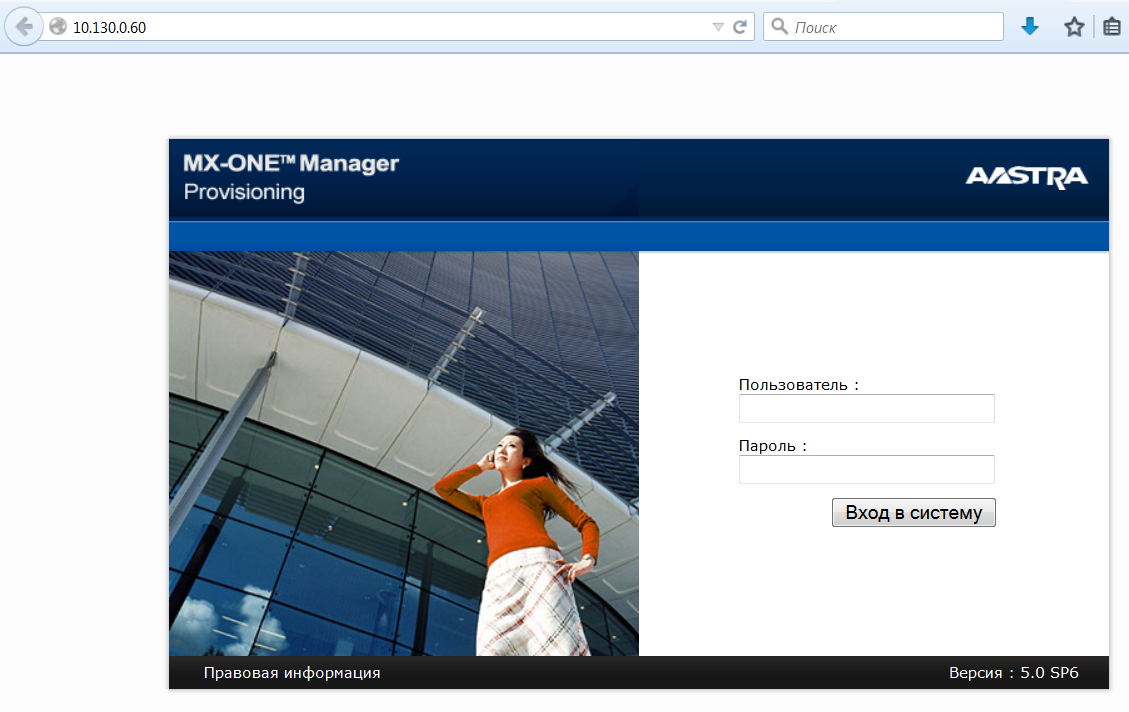
\includegraphics[width=\linewidth]{mp_login}
  \caption{Система управления Manager Provisioning}
  \label{img:mp_login}
\end{figure}
%\clearpage

Изменить подключение HTTP или HTTPS и способ аутентификации можно с помощью запуска в консоли команды {\em webserver\_config} от имени {\em root} (рис. \ref{img:web_config}).

\begin{figure}[!ht]
  \center
  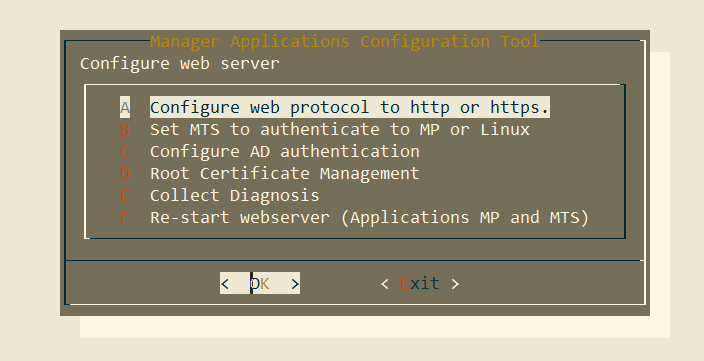
\includegraphics[width=0.7\linewidth]{web_config}
  \caption{Конфигурация веб--сервера}
  \label{img:web_config}
\end{figure}
\clearpage

Веб--интерфейс MP русифицирован, также как и подсказки к каждому полю в настройках (on--line help).
Русский язык можно включить через Главное меню {\em <<Own Settings>> $\rightarrow$ <<General>> $\rightarrow$ <<Language>>}
(рис. \ref{img:mp_lang}).
\begin{figure}[!ht]
  \center
  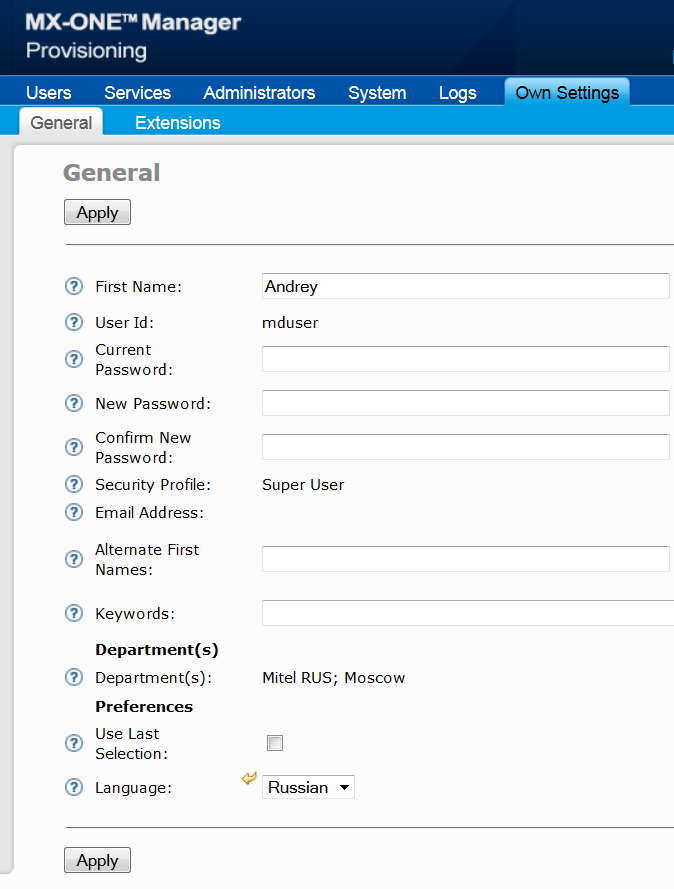
\includegraphics[width=0.7\linewidth]{mp_lang}
  \caption{Настройка русского языка в MP}
  \label{img:mp_lang}
\end{figure}
%\clearpage

После смены языка интерфейс и подсказки будут отображаться на русском языке (рис. \ref{img:mp_about}).
\begin{figure}[!ht]
  \center
  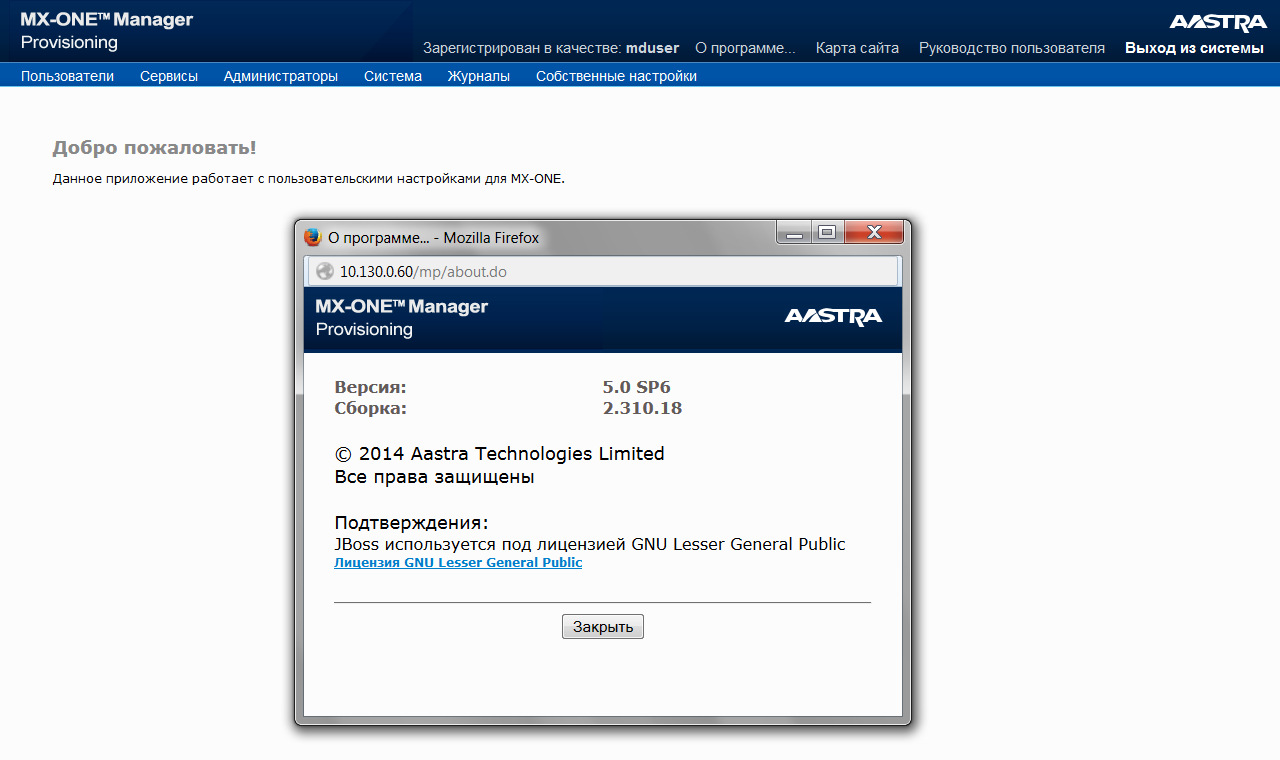
\includegraphics[width=\linewidth]{mp_about}
  \caption{ПО Manager Provisioning}
  \label{img:mp_about}
\end{figure}
%\clearpage

Manager Provisioning может централизованно выполнять конфигурацию подсистем MX--ONE. Для этого необходимо добавить управляемую подсистему через меню {\em <<Система>> $\rightarrow$ <<Подсистема>> $\rightarrow$ <<Добавить>>} (рис. \ref{img:mp_add_subsystem}).
\begin{figure}[!ht]
  \center
  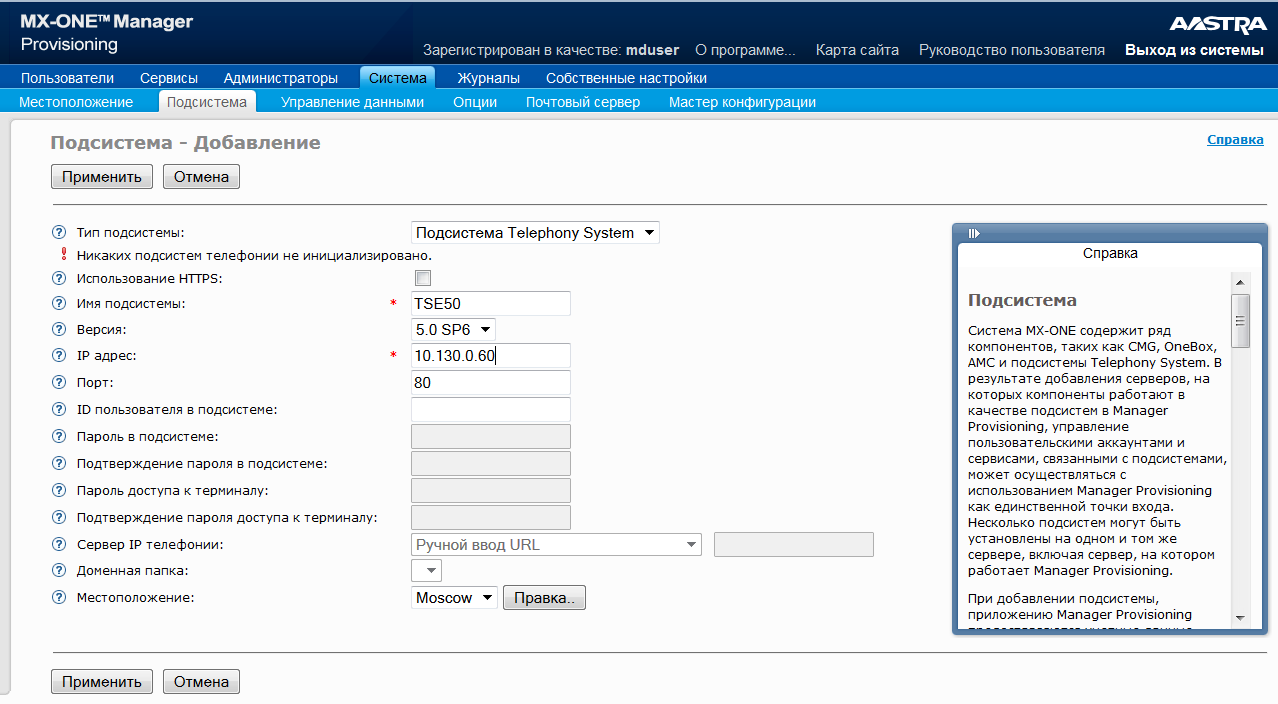
\includegraphics[width=\linewidth]{mp_add_subsystem}
  \caption{MP --- добавление подсистемы}
  \label{img:mp_add_subsystem}
\end{figure}
%\clearpage

После успешного добавления подсистемы в интерфейс MTS можно будет автоматически зайти кликнув по имени подсистемы (рис. \ref{img:mp_to_mts}).
\begin{figure}[!ht]
  \center
  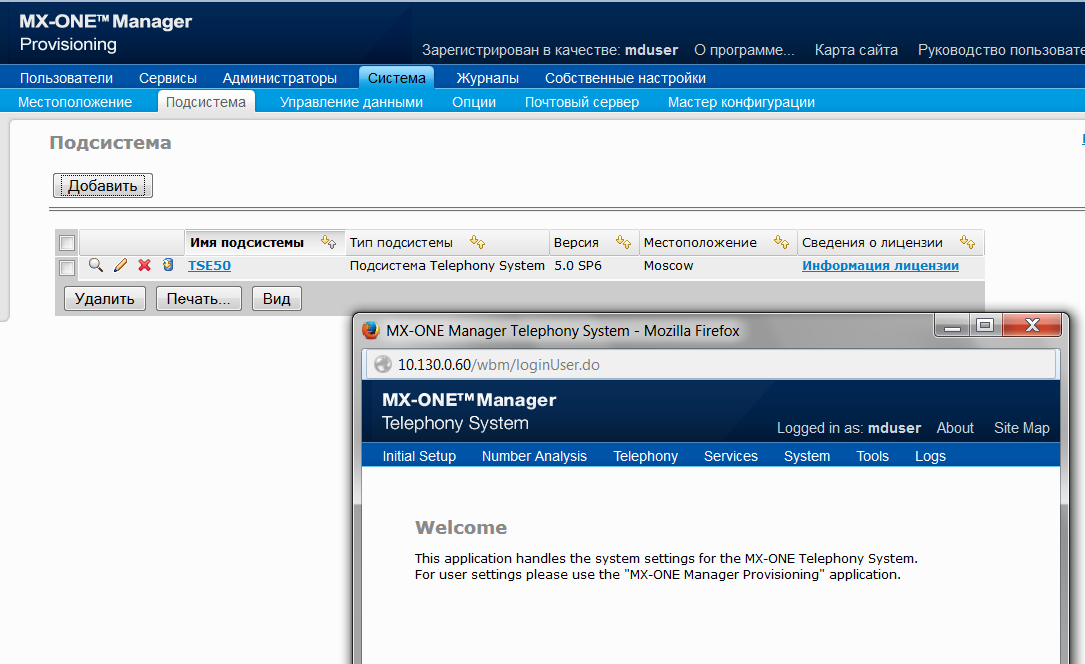
\includegraphics[width=\linewidth]{mp_to_mts}
  \caption{MP --- подсистемы}
  \label{img:mp_to_mts}
\end{figure}
\clearpage


\subsection{Конфигурация абонента в Manager Provisioning}

Если предварительно создан внутренний номерной план (раздел \ref{subsec:numbers}) и сервисный профайл (раздел \ref{subsec:csp}), то можно добавить абонентов через меню: {\em <<Сервисы>> $\rightarrow$ <<Абонент>> $\rightarrow$ <<Добавить>>} и далее выбрать доступную подсистему и тип подключаемого абонента (рис. \ref{img:add_user}).
\begin{figure}[!ht]
  \center
  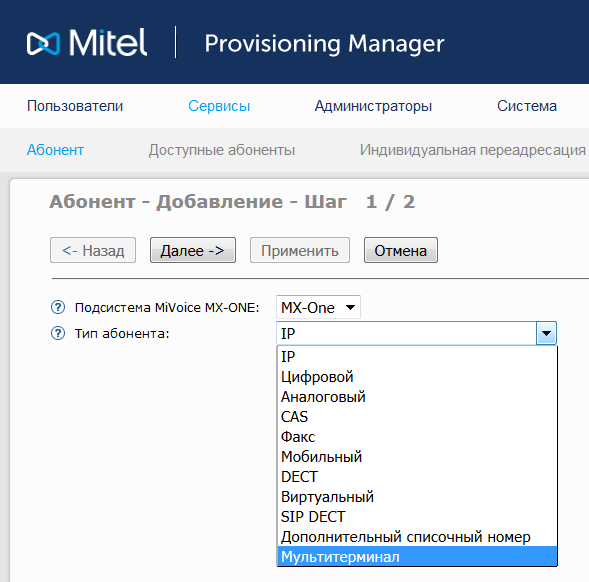
\includegraphics[width=0.7\linewidth]{add_multy}
  \caption{MP --- создание нового абонента}
  \label{img:add_user}
\end{figure}

Тип абонента может быть как цифровой, аналоговый, IP и др., а также для IP--абонентов можно выбрать тип <<Мультитерминал>>. Тип <<Мультитерминал>> позволяет подключить одновременно до 4--х разных IP--устройств на один номер. Все телефоны при входящем вызове будут звонить одновременно, ответить можно на любом, и можно передавать активный вызов между терминалами с помощью функции <<Take>>.

На следующем экране вводятся:
\begin{itemize}
  \item номер абонента из доступного диапазона;
  \item номер сервера;
  \item сервисный профайл;
  \item язык;
  \item имя и фамилия абонента;
  \item тип телефона и дополнительные панели;
  \item и другие параметры (рис. \ref{img:user1000}).
\end{itemize}

\begin{figure}[!ht]
  \center
  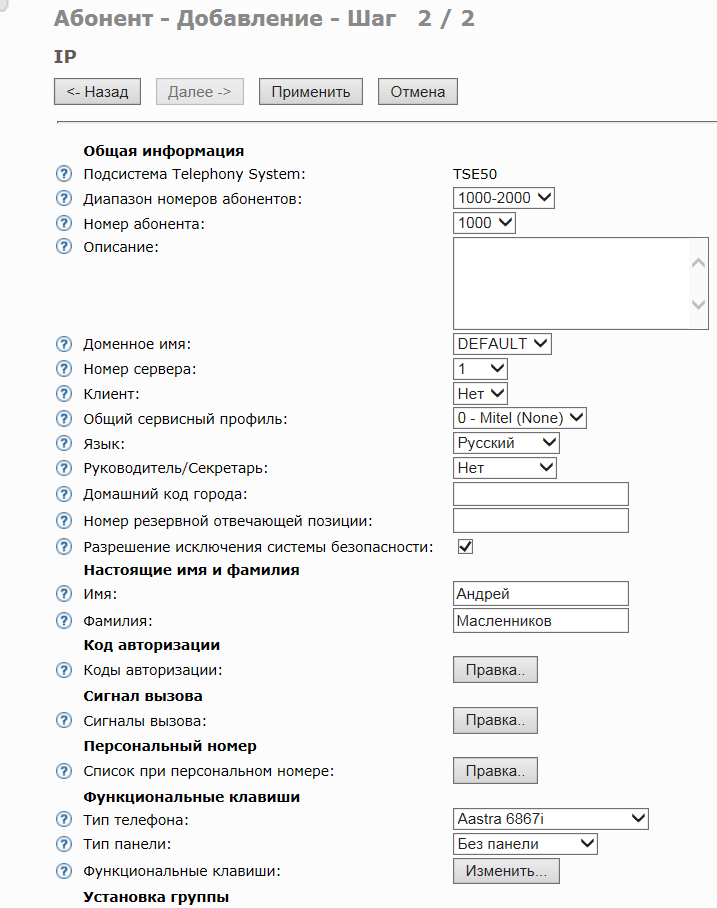
\includegraphics[width=0.9\linewidth]{user1000}
  \caption{MP --- создание нового абонента (2)}
  \label{img:user1000}
\end{figure}
\clearpage

Далее нужно подтвердить настройки, после чего можно посмотреть, отредактировать или удалить созданных абонентов (рис. \ref{img:users}).
\begin{figure}[!ht]
  \center
  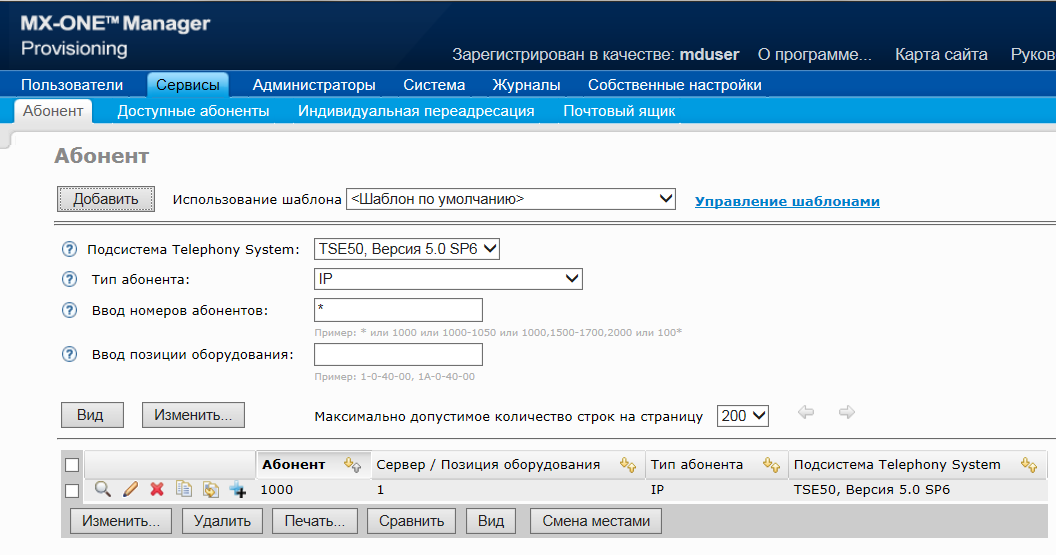
\includegraphics[width=\linewidth]{users}
  \caption{MP --- просмотр и редактирование абонентов}
  \label{img:users}
\end{figure}

Добавить возможность подключения програмного SIP--клиента Mitel BluStar for PC с возможностью передачи видео можно отметив соответствующие пункты в дополнительных настройках абонента как показано на рис. \ref{img:add_bs4pc}.
\begin{figure}[!ht]
  \center
  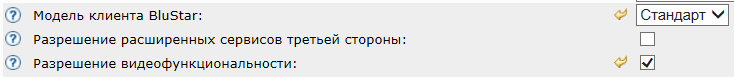
\includegraphics[width=0.9\linewidth]{add_bs4pc}
  \caption{MP --- добавление функционала BluStar for PC}
  \label{img:add_bs4pc}
\end{figure}


Далее можно уже совершать звонки между SIP-абонентами с помощью, например, софтфона BluStar for PC.

Добавить абоненту (extension \#1000) возможность подключения программного клиента BluStar for PC c опцией передачи видео можно также из командной строки:
\begin{lstlisting}
admin@TSE50:/> extension -d 1000 -c --blustar-client-model STANDARD --video 1

admin@TSE50:/> extension -p -d 1000
Directory Number Profile
Dir        Cust LIM CSP Lang Max  Secretary Max  Security  AMC Video BluStar      Third Party       Hotline Hotline Number
Backup Number        Area
Cost           Term Exception           Client Model Enhanced Services
Code
1000       0    1   0   6    -    No        1    Yes       No  Yes   STANDARD     No                -       -
\end{lstlisting}

\subsection{Конвертация IP--абонента в тип <<Мультитерминал>>}

Если тип абонента был установлен как <<IP>>, то его потом можно будет конвертировать в тип <<Мультитерминал>> нажав на значок <<+>> рядом с номером абонента в списке (рис. \ref{img:multy_dev}):
\begin{figure}[!ht]
  \center
  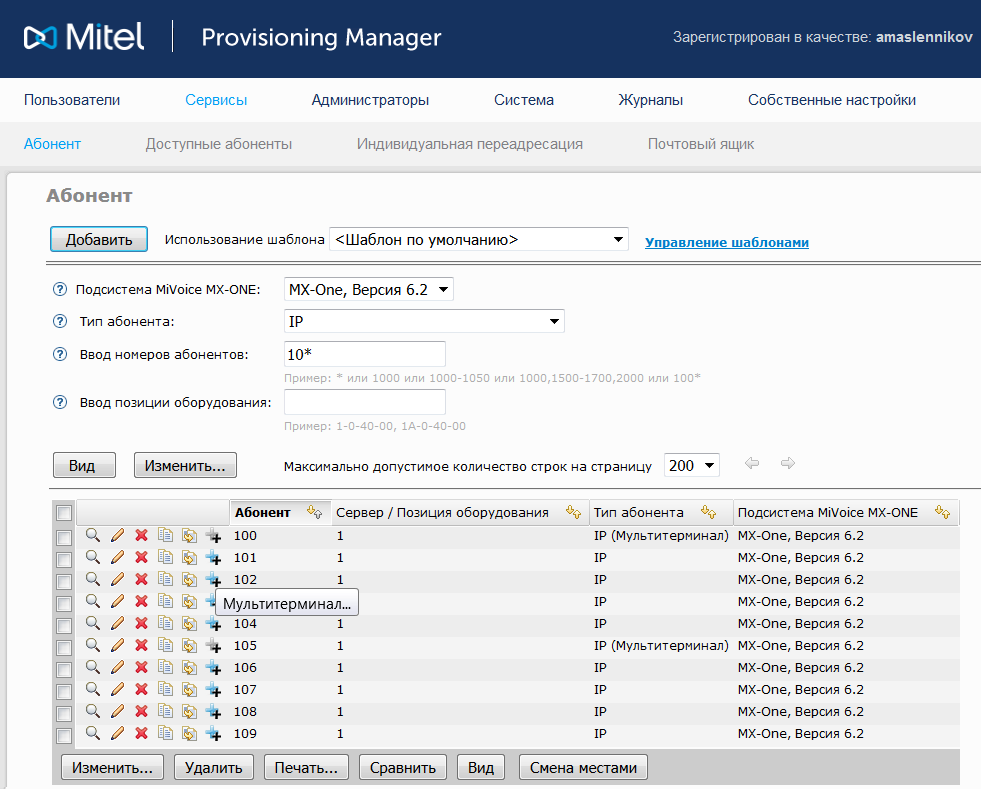
\includegraphics[width=0.9\linewidth]{multy_device}
  \caption{Конвертация IP--абонента в тип IP (Мультитерминал)}
  \label{img:multy_dev}
\end{figure}

\subsection{Настройка персонального номера}

В настройках абонента (рис. \ref{img:user1000}) есть возможность настроить <<Персональный номер>> (рис. \ref{img:personal_number}): 

\begin{figure}[!ht]
  \center
  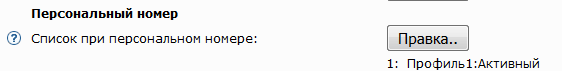
\includegraphics[width=0.7\linewidth]{personal_number}
  \caption{Настройка персонального номера}
  \label{img:personal_number}
\end{figure}

Для каждого абонента доступно до 5 персональных профилей (списков вызовов) (рис. \ref{img:personal_profile}).

\begin{figure}[!ht]
  \center
  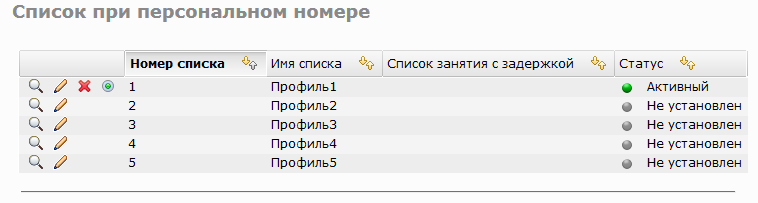
\includegraphics[width=0.9\linewidth]{personal_profile}
  \caption{Список доступных профилей}
  \label{img:personal_profile}
\end{figure}

Например, в <<Профиле 1>>, в случае если абонент с номером 105 не ответил в течение 20 секунд, то вызов перейдет на номер 124 "--- это может быть номером ящика голосовой почты (рис. \ref{img:personal_call_list}):

\begin{figure}[!ht]
  \center
  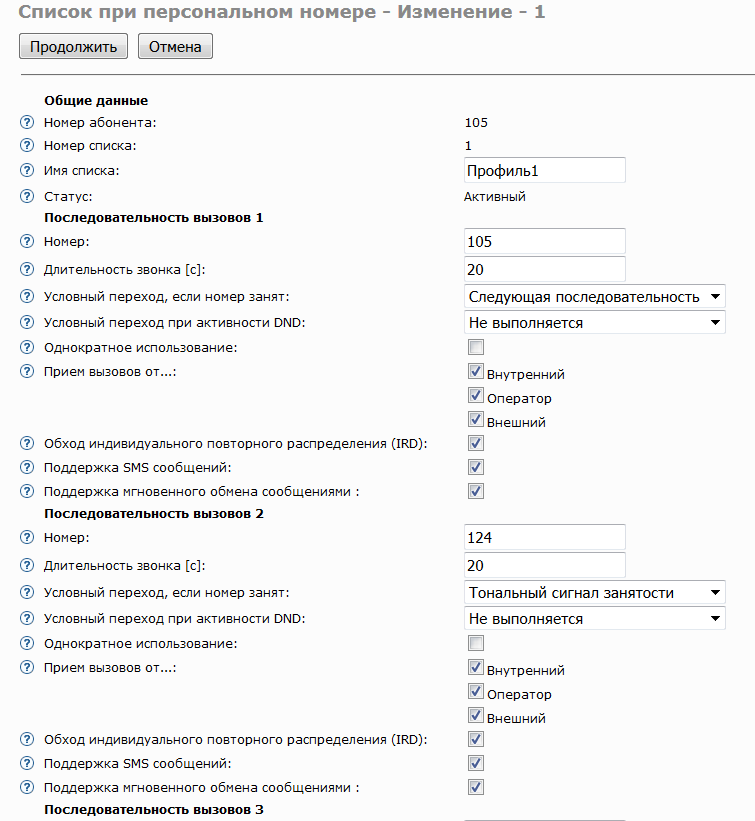
\includegraphics[width=0.9\linewidth]{personal_call_list}
  \caption{Список вызовов}
  \label{img:personal_call_list}
\end{figure}

\clearpage

\section{Настройка терминального оборудования}

\subsection{Конфигурация программного SIP-клиента BluStar for PC}

Если не настроено подключение с авторизацией, то достаточно указать номер абонента (extension) и IP--адрес SIP--сервера (порт по умолчанию 5060) как показано на рис. \ref{img:bs_config}:
\begin{figure}[!ht]
  \center
  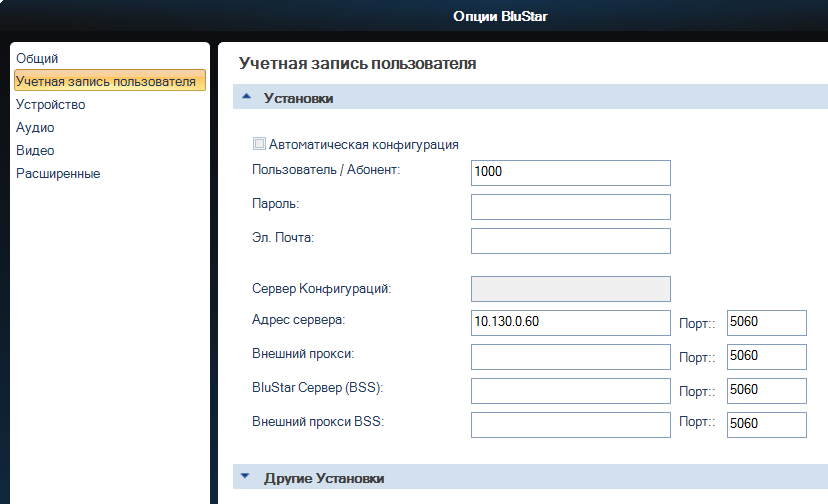
\includegraphics[width=0.9\linewidth]{bs_config}
  \caption{Настройка BluStar for PC}
  \label{img:bs_config}
\end{figure}

Для автоматической конфигурации SIP--абонентов используются следующие конфигурационные файлы, которые загружаются с конфигурационного сервера в момент загрузки софтфона:
\begin{itemize}
	\item Системная конфигурация:  aastra.cfg
	\item Конфигурация конкретной модели:  BSCpc.cfg
	\item Конфигурация конкретного пользователя {\em user}:  BSCpc\_<user>.cfg
        \item Пользовательские настройки: BSCpc\_<user>\_local.cfg
	\item Данные пользователя (контакты, история вызовов, фотографии): BSCpc\_prefs\_<user>.cfg
\end{itemize}

Файл конфигурации для модели {\em BSCpc.cfg} загружается с сервера, только если он отсутвует на клиентской машине. Локально на Windows--компьютере он хранится в папке:
\begin{lstlisting}
c:\Users\....\AppData\Roaming\Aastra\BluStar\BSCpc.cfg
\end{lstlisting}

\subsubsection{Выбор кодека}
Для выбора вариантов голосовых кодеков необходимо отредактировать файл {\em BSCpc.cfg}. 
Список доступных кодеков:
\begin{itemize}
	\item PCMU
	\item PCMA
	\item G722
	\item G729AB (only available in local markets)
	\item ILBC
	\item Default value  (none)
\end{itemize}

Чтобы выбрать из списка первые 2 кодека PCMU и PCMA нужно указать из порядковый номер начиная с нуля:
\begin{lstlisting}
telephony codecs : 0,1
\end{lstlisting}

\subsection{Настройка сервера конфигурации для SIP--телефонов}
При загрузке SIP--телефона, телефон автоматически может получать от DHCP--сервера также адрес сервера конфигурации, на котором хранятся файлы конфигурации, актуальные прошивки (firmware) и файлы локализации.
Фрагмент настройки конфигурационного сервера DHCP--сервера (isc-dhcp-server) для Linux (/etc/dhcp/dhcpd.conf):
\begin{lstlisting}
option tftp-server-name ``10.130.0.3'';

option space AastraIPPhone6869i;
option AastraIPPhone6869i.cfg-server-name code 02 = text;

subnet 10.130.0.0 netmask 255.255.255.0 {
    range 10.130.0.100 10.130.0.120;

    class ``vendor-class-6869i'' {
      match if option vendor-class-identifier=''AastraIPPhone6869i'';
      vendor-option-space AastraIPPhone6869i;
      option AastraIPPhone6869i.cfg-server-name ``tftp://10.130.0.3/aastra67xxi'';
    }
}
\end{lstlisting}

С указанного адреса TFTP--сервера SIP--телефон Mitel 6869i загрузит последнюю прошивку (6869i.st) конфигурационные файлы (aastra.cfg, 6869i.cfg) и файл локализации с русским языком (lang\_ru.txt).

\subsection{Подключение корпоративной адресной книги AD/LDAP}
На UC360 конфигурацию AD можно выполнить через экранное меню терминала {\em <<Settings>> $\rightarrow$ <<Advanced>> $\rightarrow$ <<System Setting>> $\rightarrow$ <<LDAP/AD Settings>> $\rightarrow$ <<LDAP Server Settings>>}. Пример настроек сервера AD/LDAP:
\begin{lstlisting}
  Directory Server IP: 10.130.0.7:389
  Communication Security Type: None
  User Login: secdemo\userlogin
  User Password: xxxxxxxx
  LDAP Search Base: DC=secdemo,DC=com
  LDAP Search Directory: cn=users
  LDAP Search Filter: objectCategory=person
  First Name Attribute: givenname
  Last Name Attribute: sn
  Office Number Attribute: telephoneNumber
\end{lstlisting}

После загрузки телефонного справочника из AD/LDAP в приложении <<Contacts>> UC360 появится список сотрудников, звонить которым можно одним нажатием на экран (рис.~\ref{img:uc360_ad}).

\begin{figure}[!ht]
  \center
  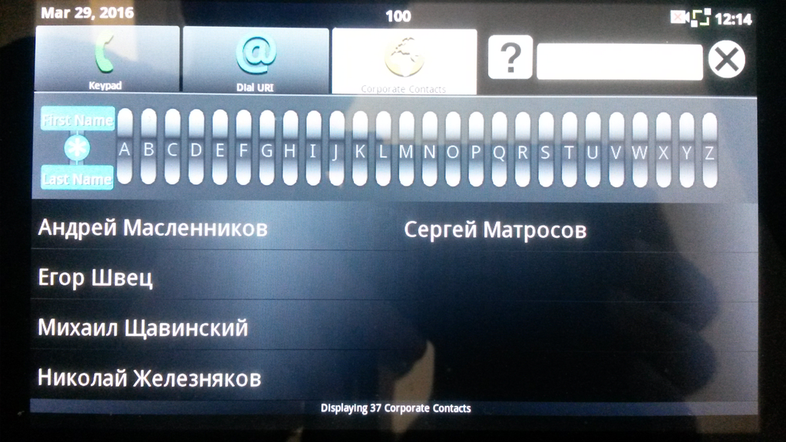
\includegraphics[width=0.7\linewidth]{uc360_ad.png}
  \caption{UC360 - Корпоративная адресная книга из AD}
  \label{img:uc360_ad}
\end{figure}


\subsection{Подключение AD/LDAP на SIP-телефонах Mitel 6800/6900}
На SIP--телефонах линейки Mitel 6800 и 6900 можно подключить адресную книгу из MS Active Directory или LDAP.

\begin{figure}[!ht]
  \center
  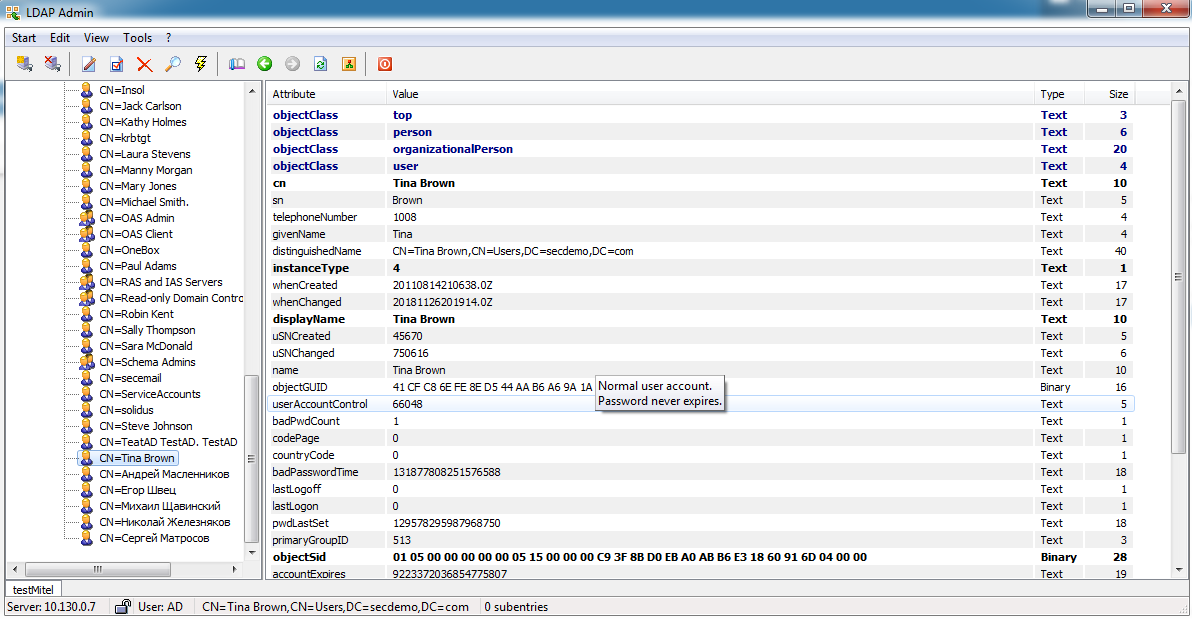
\includegraphics[width=0.9\linewidth]{ldap_admin}
  \caption{Просмотр структуры записей AD через программу LDAP Admin}
  \label{img:ldap_admin}
\end{figure}

Пример конфигурационного файла:
\begin{lstlisting}
ldap name: Mitel
ldap server:login:password@10.130.0.7:389
ldap base dn:DC=secdemo,DC=com
ldap search scope:cn=Users
ldap search filter:objectCategory=person
ldap business phone 1 attribute list:telephoneNumber
ldap downloaded:1
ldap enabled:1
directory disabled:0
softkey9 type:directory
softkey9 locked:0
\end{lstlisting}

\begin{figure}[!ht]
  \center
  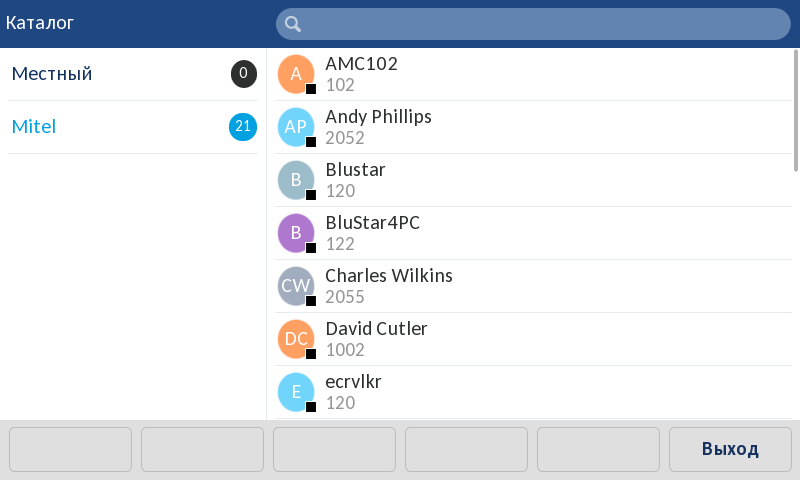
\includegraphics[width=0.7\linewidth]{ldap_phone}
  \caption{Просмотр адресной книги на телефоне}
  \label{img:ldap_phone}
\end{figure}

\subsection{XML--сервисы на SIP--телефонах}
Схема подключения корпоративных адресных книг AD/LDAP через XML--прокси сервер (рис. \ref{img:xml_proxy}).
\begin{figure}[!ht]
  \center
  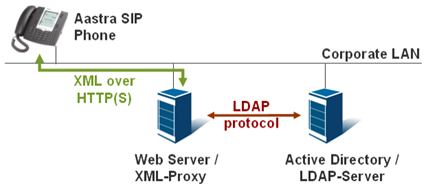
\includegraphics[width=0.7\linewidth]{XML_proxy}
  \caption{Схема подключения корпоративной адресной книги на телефоне}
  \label{img:xml_proxy}
\end{figure}
 
Добавление ссылки на XML--сервер в web--интерфейсе SIP--телефона {\em <<Операции>> $\rightarrow$ <<Софтклавиши и XML>>} (рис. \ref{img:xml_config}).
\begin{figure}[!ht]
  \center
  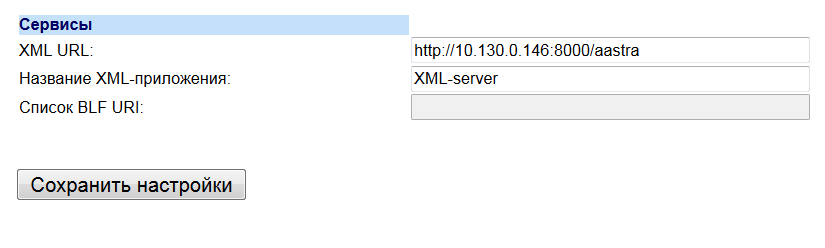
\includegraphics[width=0.9\linewidth]{xml_config}
  \caption{Настройка XML--сервера на телефоне}
  \label{img:xml_config}
\end{figure}

Логин/пароль для администрирования SIP--телефонов Mitel серии 6700/6800 по умолчанию: {\em admin/22222}.

Пример XML--меню на телефоне 6739i (рис. \ref{img:xml_menu}).
\begin{figure}[!ht]
  \center
  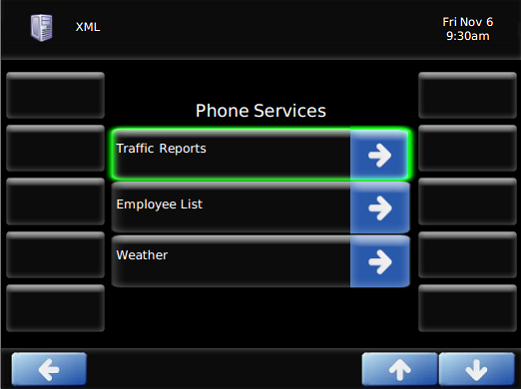
\includegraphics[width=0.7\linewidth]{xml_menu}
  \caption{Пример XML--меню на телефоне}
  \label{img:xml_menu}
\end{figure}
 
\subsubsection{Отправка push XML--сообщения}

Пример XML-файла textscreen.xml:
\begin{lstlisting}
xml=<AastraIPPhoneTextScreen>
<Title>Phone Services</Title>
<Text>Hello Mitel!</Text>
</AastraIPPhoneTextScreen>
\end{lstlisting}

Пример команды для отправки XML--сообщения на телефон:
\begin{lstlisting}
#curl -H "Content-Type: text/xml" -X POST -d @textscreen.xml http://10.130.0.108
\end{lstlisting}

Разрешение отправки XML push--сообщений с IP--адреса сервера через web--интерфейс телефона: 
{\em <<Расширенные настройки>> $\rightarrow$ <<Настройки сервера конфигурации>>} (рис. \ref{img:xml_push}). 
\begin{figure}[!ht]
  \center
  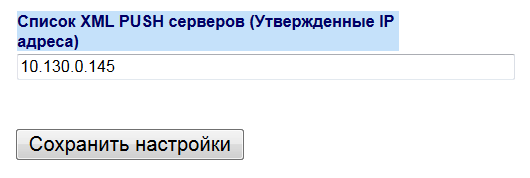
\includegraphics[width=0.7\linewidth]{xml_push}
  \caption{Настройка push--уведомлений на телефоне}
  \label{img:xml_push}
\end{figure}

\subsection{Настройка отображения фотографии звонящего на SIP--телефонах Mitel 6700/6800}

Для отображения фотографии звонящего на телефоне необходимо добавить строку с адресом сервера c фотографиями в конфигурационный файл $aastra.cfg$: 
\begin{lstlisting}
image server uri: tftp://10.130.0.3
\end{lstlisting}

Фотографии абонентов нужно сохранить в соответствующую директорию на сервере в формате $png$. Именем файла должен являться номер абонента: 
\begin{lstlisting}
mxone_admin@MX-One6:/tftpboot> ls -1
100.png
101.png
102.png
103.png
104.png
105.png
\end{lstlisting}

После этого на экране телефона при входящем или исходящем звонке будет отображаться фотография абонента рис. \ref{img:call_photo}:
\begin{figure}[!ht]
  \center
  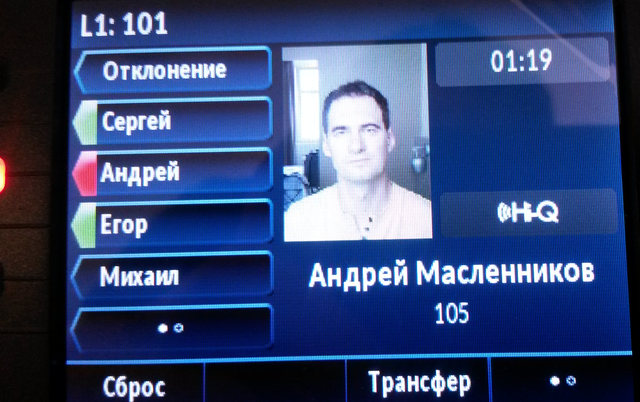
\includegraphics[width=0.7\linewidth]{call_photo}
  \caption{Отображение фотографии звонящего}
  \label{img:call_photo}
\end{figure}

\section{Контроль состояния системы}

\subsection{Команды для мониторинга}

Для вывода списка активных аварий на станции можно воспользоваться командой {\em alarm -p}:
\begin{lstlisting}
eri_sn_admin@:~> alarm -p

Global status: Severity0:78-0, S1:6-0, S2:2-0, S3:0-0, S4:0-0, High=2
No erase/reset of alarms done

S N    Handle  Dom.  Code LIM Where        Explanation
=============================================================================
2        2177     0   274   1 SLP60        DIGITAL TRUNK, CLOCK MALFUNCTION (SLIP)
2        8065     0   303   1 SLP60        DATA LINK ALARM
1         385     0    45   1              LIM reloaded and restarted
1         897     0    40   1 SYSSAM       Exchange data reloaded
1        1025     1    23   1              Rollback of ldap data successful
1        3329     0    30   1 AL           Incrementation alarm for alarm severity 0
1        3713     0    40   1 AMP-user     Exchange data reloaded
1        5377     0    40   1 AMP-user     Exchange data reloaded
0         129     0    65   1 MGW 1A       Synchronization fault in LIM
0         257     0    65   1 MGW 1A       Synchronization fault in LIM
0         513     0   303   1 SLP60        DATA LINK ALARM
0         641     0    15   1 001A-0-20    Device board faulty or missing
0         769     0   363   1 001A-0-70    IP device board, major fault
\end{lstlisting}

Команда выводит список аварий отсортированный по степени серьезности <<S>>. Наивысший уровень 6, а низший уровень 0 --- значит, что авария уже снята и её можно стереть из списка командой {\em alarm -e}. В списке указан номер подсистемы, где произошла авария в поле <<LIM>>, название программного модуля или позиции платы в поле <<Where>> и дано краткое описание аварии.

Подробные данные можно получить задав полный формат вывода командой {\em alarm -p -f full}.

Информацию о доступных маршрутах можно посмотреть перейдя в командную оболочку {\em mdsh} и вывести список командой {\em rodap:rou=all;} :  
\begin{lstlisting}
eri_sn_admin@:~> mdsh
MDSH> rodap:rou=all;
ROUTE DATA
ROU   TYPE  VARC        VARI        VARO        FILTER
1     TL66  H'00000000  H'00000000  H'00000104  NO
2     TL66  H'00000000  H'00000000  H'00000051  NO
3     TL66  H'00000000  H'00000000  H'00000111  NO
9
11    TL66  H'00000000  H'00000000  H'00000000  NO
35    TL66  H'00000000  H'00000000  H'00000000  NO
37    TL66  H'00000000  H'00000000  H'00000000  NO
38    TL66  H'00000000  H'00000000  H'00000114  NO
46    TL66  H'00000000  H'00000000  H'00000000  NO
60    SL60  H'00000300  H'00000002  H'06410000  NO
70    SL60  H'00100300  H'00010000  H'06310000  NO
79    SL60  H'00000230  H'05400000  H'06310000  NO
100   TL66  H'00000000  H'00000000  H'00000000  NO
150   TL65  H'00000001  H'00000001  H'00000000  NO

END
\end{lstlisting}

В списке указан номер маршрута <<ROU>> и его тип. Тип <<TL66>> соответствует SIP, <<SL60>> --- ISDN-E1, а <<TL65>> --- H.323.

Состояние транков (каналов) в конкретном маршруте типа ISDN-E1 выдается следующей командой:
\begin{lstlisting}
MDSH> susip:rou=60,tru=all;
STATUS INFORMATION AT 14:05 14AUG15
ROU  TRU       TYPE   TRAFFIC STATE/PTR    LINE STATE/PTR     ADD INFO
60   001-1     TL60   IDLE          #0000  FREE       #0006
60   001-2     TL60   IDLE          #0001  FREE       #0007
60   001-3     TL60   IDLE          #0002  FREE       #0008
60   001-4     TL60   IDLE          #0003  FREE       #0009
60   001-5     TL60   IDLE          #0004  FREE       #000A
60   001-6     TL60   IDLE          #0005  FREE       #000B
60   001-7     TL60   IDLE          #0006  FREE       #000C
60   001-8     TL60   IDLE          #0007  FREE       #000D
60   001-9     TL60   IDLE          #0008  FREE       #000E
60   001-10    TL60   SPEECH        #0009  BUSY       #000F
END
\end{lstlisting}

В листинге видно, что некоторые каналы свободны (IDLE/FREE), а некоторые заняты разговором (SPEECH/BUSY). 

Состояние регистрации SIP--абонентов в системе можно посмотреть командой {\em ip\_extension\_info}:
\begin{lstlisting}
eri_sn_admin@TSE50:~> ip_extension_info
IP Extension Info
Dir          Cust   LIM   IP Address            RAS     CS
Port    Port
1000         0      -     Not registered        -       -

eri_sn_admin@TSE50:~> ip_extension_info
IP Extension Info
Dir          Cust   LIM   IP Address            RAS     CS
Port    Port
1000         0      1     10.130.0.145          -       49798
\end{lstlisting}

В случае успешной регистрации в листинге видно номер абонента (1000), его IP--адрес и номер порта.

\subsection{Трассировка вызова} \label{subsec:trace}

Для трассировки вызовов служит команда $call\_trace$. Например, для номера 103 трассировка вызова будет выглядеть так:
\begin{lstlisting}
  MX-One6:~ # call_trace -d 103
  Number 103 is a generic number.

  SIP extension
  sip:103@10.130.0.83;instance=urn:uuid:00000000-0000-1000-8000-00085D13CAC9

  *************************************************************
  State is: SPEECH
  -------------------------------------------------------------
  Start time: 2015-10-23 14:03:54 (EET) Duration: 0d00:00:02
  Call type: 8 (Ordinary internal call)
  A-number (int): 101                   Charged : 101
  Dialled-number: 103                   Called  : 103

  Connection type: pointToPoint
  --------------------------------
  A_Party in  Lim:   1, Unit: SIPLP          {MD_Type::Address lim=1, unit=0x12a, pointer=0xd7ad, addrCtrl=0xa2}
  Party RTP address:   10.130.0.82:3000, Codec: (audio(0)-G722)
  Direct media
  --------------------------------
  B_Party1 in Lim:   1, Unit: SIPLP          {MD_Type::Address lim=1, unit=0x12a, pointer=0xd7ae, addrCtrl=0xa6}
  Party RTP address:   10.130.0.83:3000, Codec: (audio(0)-G722)
  Direct media
  --------------------------------
\end{lstlisting}

На листинге выше видно установление RTP--соединения (кодек G.722) между абонентами 101 и 103 напрямую между IP--адресами 10.130.0.82 и 10.130.0.83.

Если была включена опция <<Forced Gateway>> (\ref{subsec:forced}), то будут установлены 2 RTP--соединения через медиа--шлюз:
\begin{lstlisting}
  MX-One6:~ # call_trace -d 103
  Number 103 is a generic number.

  SIP extension
  sip:103@10.130.0.83;instance=urn:uuid:00000000-0000-1000-8000-00085D13CAC9

  *************************************************************
  State is: SPEECH
  -------------------------------------------------------------
  Start time: 2015-10-23 13:59:04 (EET) Duration: 0d00:04:34
  Call type: 8 (Ordinary internal call)
  A-number (int): 101                   Charged : 101
  Dialled-number: 103                   Called  : 103

  Connection type: pointToPoint
  --------------------------------
  A_Party in  Lim:   1, Unit: SIPLP          {MD_Type::Address lim=1, unit=0x12a, pointer=0xd79c, addrCtrl=0x89}
  Party RTP address:   10.130.0.82:3000, Codec: (audio(0)-PCMA)
  Gateway RTP address:    10.130.0.8:40146, Codec: (audio(0)-PCMA), Multiple:   1A-0-40-20
  --------------------------------
  B_Party1 in Lim:   1, Unit: SIPLP          {MD_Type::Address lim=1, unit=0x12a, pointer=0xd79d, addrCtrl=0x8d}
  Party RTP address:   10.130.0.83:3000, Codec: (audio(0)-PCMA)
  Gateway RTP address:    10.130.0.8:40144, Codec: (audio(0)-PCMA), Multiple:   1A-0-40-19
  LS connection
  Mult-x  :   1A-0-40-19, Attenuation: x->y=2
  Mult-y  :   1A-0-40-20, Attenuation: y->x=2
  --------------------------------
\end{lstlisting}

На листинге выше видно установление двух соединений (кодек G.711) через медиа--шлюз 1A по адресу 10.130.0.8.

\subsection{SNMP--мониторинг и управление}

С помощью встроенного SNMP--агента MX--ONE TSE может отправлять сообщения об авариях, изменениях статусов, а также в ответ на запросы сетевой системы управления (NMS) изменять параметры конфигурации и сообщать информацию о состоянии системы. Можно также настроить оправку сообщений об авариях на e--mail или SMS. База управляющей информации описана в MIB--файле. 
\nomenclature{\ MIB}{--- Management Information Bases (База управляющей информации)}
MIB--файл с полным описанием доступных переменных можно найти в файловой системе MX--ONE:
\begin{lstlisting}
/usr/share/snmp/mibs/MX-ONE-TS-ALARM-MIB.txt
\end{lstlisting}

В структуре MIB за Mitel (Aastra) MX--ONE TS зарезервирован специальный идентификатор объекта OID
в числовом виде:
\begin{lstlisting}
.1.3.6.1.4.1.11268.2.8
\end{lstlisting}
или в текстовом виде:
\begin{lstlisting}
iso(1).org(3).dod(6).internet(1).private(4).enterprises(1).aastra(11268).
aastraMibs(2).aastraOidMx-one(8).tsAlarm(1).tsObjects(2)
\end{lstlisting}
который используется для доступа к информации. 

В MX--ONE 5.0 для доступа только к базовым объектам tsAlarm(1).tsAlarmR1(1) MIB требуется лицензия SNMP--Basic, а для доступа ко всем объектам включая tsAlarm(1).tsObjects(2) необходима лицензия SMNP--Advanced.

В MX--ONE 6.0 есть только одна лицензия SNMP--Advanced.

На рис. \ref{img:nms} показан пример графического интерфейса SNMP--модуля MX--ONE для NMS HP OpenView.
\begin{figure}[!ht]
  \center
  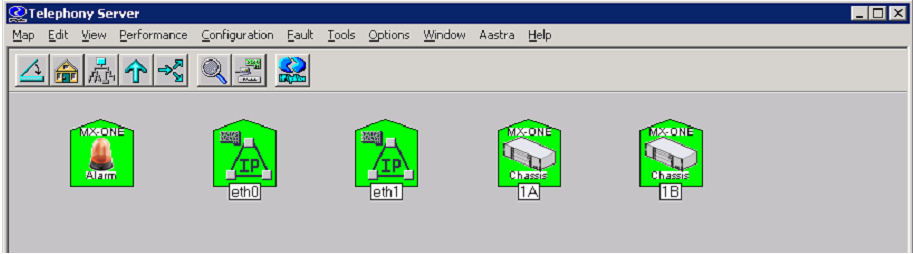
\includegraphics[width=0.9\linewidth]{nms}
  \caption{MX-ONE SNMP 5.0 Plug-in for HP Openview 7.53}
  \label{img:nms}
\end{figure}

\subsection{Система контроля производительности -- Mitel Performance Analytics}
\nomenclature{\ MPA}{--- Mitel Performance Analytics}

Начиная с версии MX-ONE 6.0 SP2 поддерживается система контроля производительности MPA, которая позволяет централизованно собирать и вести журнал аварий со всех серверов в системе, создавать отчёты, рассылать уведомления, обеспечивает удалённый доступ, содержит средства удаленной сетевой диагностики, а также позволяет контролировать качество передачи голоса VoIP при каждом вызове. Система MPA состоит из центрального сервера и удалённых пробов, работающих на Java Virtual Machine.

На MX-ONE необходимо настроить отправку SNMP--traps на IP--адрес проба:
\begin{lstlisting}
mxone_user@MX-One6:~> cat /etc/snmp/snmpd.conf
syslocation Server Room
syscontact Sysadmin (root@localhost)
rocommunity public
master agentx
AgentXSocket tcp:localhost:705
trapcommunity public
trap2sink 10.130.0.33
\end{lstlisting}

В конфигурационный файл SIP--телефонов Mitel (aastra.cfg) необходимо добавить строки конфигурации для отправки RTCP--отчётов о качестве голоса также на IP--адрес проба:
\begin{lstlisting}
sip rtcp summary reports: 1
sip rtcp summary report collector: collector@10.130.0.33
sip rtcp summary report collector port: 5060
\end{lstlisting}

На рис. \ref{img:mpa} показан пример графического интерфейса Mitel Performance Analytics.
\begin{figure}[!ht]
  \center
  \includegraphics[width=0.9\linewidth]{mpa}
  \caption{Mitel Performance Analytics}
  \label{img:mpa}
\end{figure}

На рис. \ref{img:r-factor} показан пример отчета о качестве голоса с оценкой R--factor по каждому вызову.
\begin{figure}[!ht]
  \center
  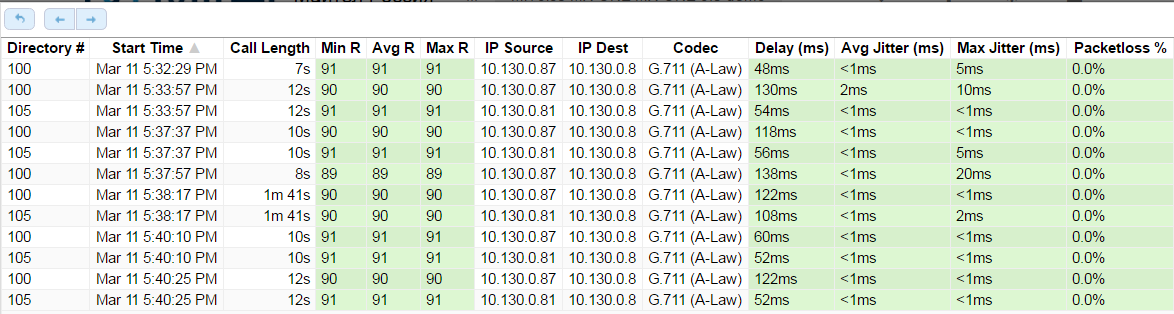
\includegraphics[width=\linewidth]{r-factor}
  \caption{Контроль качества голоса VoIP}
  \label{img:r-factor}
\end{figure}

Также мы можем контролировать уровень нагрузки на медиа--шлюзы. На  рис. \ref{img:mgw_util} мы видим среднее кол-во вызовов в час (CPH, call per hour) и процент занятых каналов от общего числа доступных ресурсов на шлюзе.  
\begin{figure}[!ht]
  \center
  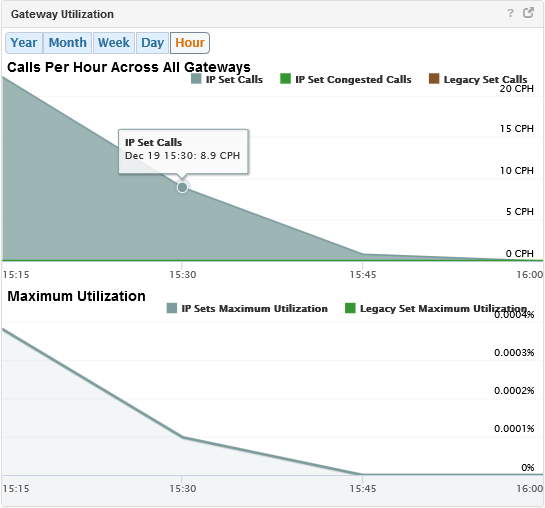
\includegraphics[width=0.7\linewidth]{mgw_util}
  \caption{Мониторинг загрузки медиа--шлюза (сервера)}
  \label{img:mgw_util}
\end{figure}

На рис. \ref{img:sip_reg} показан пример мониторинга зарегистрированных SIP--терминалов и номеров (extentions). Кол-во терминалов может быть больше зарегистрированных номеров, т.к. используется номера с функцией <<Мультитерминал>>.
\begin{figure}[!ht]
  \center
  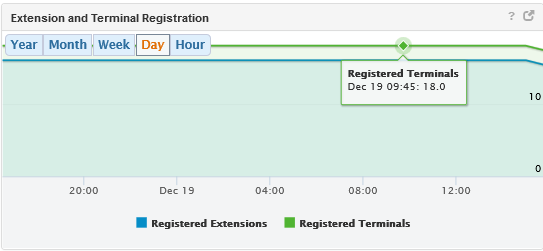
\includegraphics[width=0.7\linewidth]{sip_registered}
  \caption{Мониторинг регистрации SIP--терминалов}
  \label{img:sip_reg}
\end{figure}

\begin{figure}[!ht]
  \center
  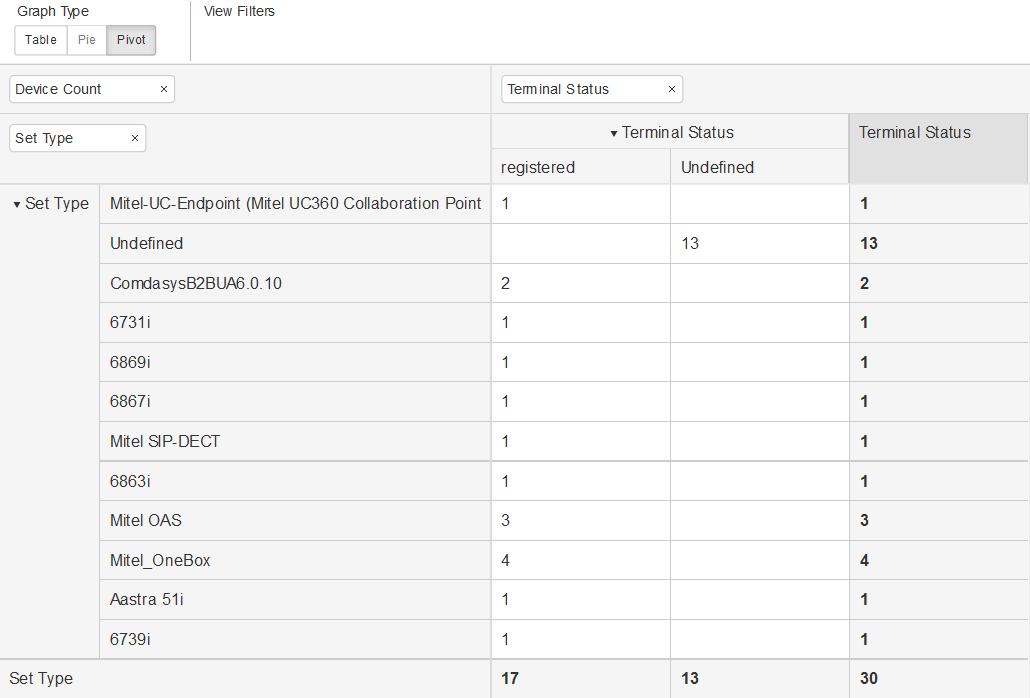
\includegraphics[width=0.9\linewidth]{sip_reg_table}
  \caption{Общая таблица регистрации по типу SIP--терминала}
  \label{img:sip_reg_table}
\end{figure}

По каждому номеру SIP возможно посмотреть подробную информацию и статусе регистрации и качестве состоявшихся разговоров (рис. \ref{img:sip_ext_123}).
\begin{figure}[!ht]
  \center
  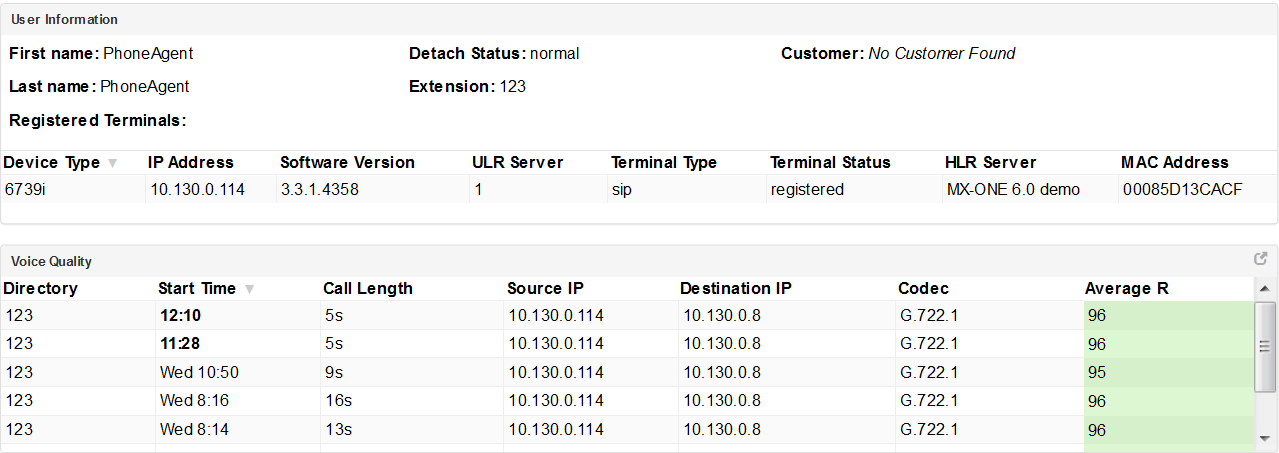
\includegraphics[width=\linewidth]{sip_ext_123}
  \caption{Статус регистрации и статистика вызовов SIP--терминала с номером 123}
  \label{img:sip_ext_123}
\end{figure}

\begin{thebibliography}{9}
  \bibitem{miteldocs} Техническая документация и прошивки для телефонов Mitel --- \href{http://miteldocs.com}{miteldocs.com}
  \bibitem{sles} SUSE Linux Enterprise Server --- \href{https://www.suse.com/ru-ru/products/server/}{suse.com}
  \bibitem{vmware} VMware ESXi --- \href{http://www.vmware.com/products/vsphere-hypervisor/}{vmware.com}
  \bibitem{yanovsky1} Яновский Г.Г., Качество обслуживания сетях IP, <<Вестник связи>>, №1, 2008 --- \href{http://niits.ru/public/2008/2008-006.pdf}{http://niits.ru/public/2008/2008-006.pdf}
  \bibitem{yanovsky2} Яновский Г.Г., Оценка качества передачи речи в сетях IP, <<Вестник связи>>, №2, 2008 --- \href{http://niits.ru/public/2008/2008-008.pdf}{http://niits.ru/public/2008/2008-008.pdf}
  \bibitem{admin_guide} Mitel MX--ONE 7.1 CPI: Administrator User's Guide --- OPERATIONAL DIRECTIONS.
\end{thebibliography}
            % Глава 1
%\input{part2}                   % Глава 2


%\bibliography{biblio}          % Подключаем BibTeX-базы
%\addcontentsline{toc}{chapter}{\bibname}   % Добавляем список
                                            % литературы в оглавление
                                            \clearpage
                                            \newpage

\listoffigures                             % Список изображений
\addcontentsline{toc}{chapter}{\listfigurename}  % Добавляем на него

%\listoftables           % Список таблиц
%\addcontentsline{toc}{chapter}{\listtablename} % Добавляем на него ссылку в оглавление

%\lstlistoflistings
%\addcontentsline{toc}{chapter}{\lstlistlistingname}

%\input{appendix}                % Приложения

\newpage
\thispagestyle{empty}

\vspace{150mm}

{\tiny Вся информация предоставляется в исходном виде, без гарантий полноты или своевременности. Использование содержимого осуществляются исключительно по вашему усмотрению и на ваш риск. Любые торговые марки, знаки и названия товаров, которые упоминаются, принадлежат их законным владельцам.}

\end{document}

